% Options for packages loaded elsewhere
\PassOptionsToPackage{unicode}{hyperref}
\PassOptionsToPackage{hyphens}{url}
%
\documentclass[
]{book}
\usepackage{lmodern}
\usepackage{amsmath}
\usepackage{ifxetex,ifluatex}
\ifnum 0\ifxetex 1\fi\ifluatex 1\fi=0 % if pdftex
  \usepackage[T1]{fontenc}
  \usepackage[utf8]{inputenc}
  \usepackage{textcomp} % provide euro and other symbols
  \usepackage{amssymb}
\else % if luatex or xetex
  \usepackage{unicode-math}
  \defaultfontfeatures{Scale=MatchLowercase}
  \defaultfontfeatures[\rmfamily]{Ligatures=TeX,Scale=1}
\fi
% Use upquote if available, for straight quotes in verbatim environments
\IfFileExists{upquote.sty}{\usepackage{upquote}}{}
\IfFileExists{microtype.sty}{% use microtype if available
  \usepackage[]{microtype}
  \UseMicrotypeSet[protrusion]{basicmath} % disable protrusion for tt fonts
}{}
\makeatletter
\@ifundefined{KOMAClassName}{% if non-KOMA class
  \IfFileExists{parskip.sty}{%
    \usepackage{parskip}
  }{% else
    \setlength{\parindent}{0pt}
    \setlength{\parskip}{6pt plus 2pt minus 1pt}}
}{% if KOMA class
  \KOMAoptions{parskip=half}}
\makeatother
\usepackage{xcolor}
\IfFileExists{xurl.sty}{\usepackage{xurl}}{} % add URL line breaks if available
\IfFileExists{bookmark.sty}{\usepackage{bookmark}}{\usepackage{hyperref}}
\hypersetup{
  pdftitle={Analyzing single-case data with R and scan},
  pdfauthor={Jürgen Wilbert},
  hidelinks,
  pdfcreator={LaTeX via pandoc}}
\urlstyle{same} % disable monospaced font for URLs
\usepackage[a4paper]{geometry}
\usepackage{color}
\usepackage{fancyvrb}
\newcommand{\VerbBar}{|}
\newcommand{\VERB}{\Verb[commandchars=\\\{\}]}
\DefineVerbatimEnvironment{Highlighting}{Verbatim}{commandchars=\\\{\}}
% Add ',fontsize=\small' for more characters per line
\usepackage{framed}
\definecolor{shadecolor}{RGB}{248,248,248}
\newenvironment{Shaded}{\begin{snugshade}}{\end{snugshade}}
\newcommand{\AlertTok}[1]{\textcolor[rgb]{0.94,0.16,0.16}{#1}}
\newcommand{\AnnotationTok}[1]{\textcolor[rgb]{0.56,0.35,0.01}{\textbf{\textit{#1}}}}
\newcommand{\AttributeTok}[1]{\textcolor[rgb]{0.77,0.63,0.00}{#1}}
\newcommand{\BaseNTok}[1]{\textcolor[rgb]{0.00,0.00,0.81}{#1}}
\newcommand{\BuiltInTok}[1]{#1}
\newcommand{\CharTok}[1]{\textcolor[rgb]{0.31,0.60,0.02}{#1}}
\newcommand{\CommentTok}[1]{\textcolor[rgb]{0.56,0.35,0.01}{\textit{#1}}}
\newcommand{\CommentVarTok}[1]{\textcolor[rgb]{0.56,0.35,0.01}{\textbf{\textit{#1}}}}
\newcommand{\ConstantTok}[1]{\textcolor[rgb]{0.00,0.00,0.00}{#1}}
\newcommand{\ControlFlowTok}[1]{\textcolor[rgb]{0.13,0.29,0.53}{\textbf{#1}}}
\newcommand{\DataTypeTok}[1]{\textcolor[rgb]{0.13,0.29,0.53}{#1}}
\newcommand{\DecValTok}[1]{\textcolor[rgb]{0.00,0.00,0.81}{#1}}
\newcommand{\DocumentationTok}[1]{\textcolor[rgb]{0.56,0.35,0.01}{\textbf{\textit{#1}}}}
\newcommand{\ErrorTok}[1]{\textcolor[rgb]{0.64,0.00,0.00}{\textbf{#1}}}
\newcommand{\ExtensionTok}[1]{#1}
\newcommand{\FloatTok}[1]{\textcolor[rgb]{0.00,0.00,0.81}{#1}}
\newcommand{\FunctionTok}[1]{\textcolor[rgb]{0.00,0.00,0.00}{#1}}
\newcommand{\ImportTok}[1]{#1}
\newcommand{\InformationTok}[1]{\textcolor[rgb]{0.56,0.35,0.01}{\textbf{\textit{#1}}}}
\newcommand{\KeywordTok}[1]{\textcolor[rgb]{0.13,0.29,0.53}{\textbf{#1}}}
\newcommand{\NormalTok}[1]{#1}
\newcommand{\OperatorTok}[1]{\textcolor[rgb]{0.81,0.36,0.00}{\textbf{#1}}}
\newcommand{\OtherTok}[1]{\textcolor[rgb]{0.56,0.35,0.01}{#1}}
\newcommand{\PreprocessorTok}[1]{\textcolor[rgb]{0.56,0.35,0.01}{\textit{#1}}}
\newcommand{\RegionMarkerTok}[1]{#1}
\newcommand{\SpecialCharTok}[1]{\textcolor[rgb]{0.00,0.00,0.00}{#1}}
\newcommand{\SpecialStringTok}[1]{\textcolor[rgb]{0.31,0.60,0.02}{#1}}
\newcommand{\StringTok}[1]{\textcolor[rgb]{0.31,0.60,0.02}{#1}}
\newcommand{\VariableTok}[1]{\textcolor[rgb]{0.00,0.00,0.00}{#1}}
\newcommand{\VerbatimStringTok}[1]{\textcolor[rgb]{0.31,0.60,0.02}{#1}}
\newcommand{\WarningTok}[1]{\textcolor[rgb]{0.56,0.35,0.01}{\textbf{\textit{#1}}}}
\usepackage{longtable,booktabs}
\usepackage{calc} % for calculating minipage widths
% Correct order of tables after \paragraph or \subparagraph
\usepackage{etoolbox}
\makeatletter
\patchcmd\longtable{\par}{\if@noskipsec\mbox{}\fi\par}{}{}
\makeatother
% Allow footnotes in longtable head/foot
\IfFileExists{footnotehyper.sty}{\usepackage{footnotehyper}}{\usepackage{footnote}}
\makesavenoteenv{longtable}
\usepackage{graphicx}
\makeatletter
\def\maxwidth{\ifdim\Gin@nat@width>\linewidth\linewidth\else\Gin@nat@width\fi}
\def\maxheight{\ifdim\Gin@nat@height>\textheight\textheight\else\Gin@nat@height\fi}
\makeatother
% Scale images if necessary, so that they will not overflow the page
% margins by default, and it is still possible to overwrite the defaults
% using explicit options in \includegraphics[width, height, ...]{}
\setkeys{Gin}{width=\maxwidth,height=\maxheight,keepaspectratio}
% Set default figure placement to htbp
\makeatletter
\def\fps@figure{htbp}
\makeatother
\setlength{\emergencystretch}{3em} % prevent overfull lines
\providecommand{\tightlist}{%
  \setlength{\itemsep}{0pt}\setlength{\parskip}{0pt}}
\setcounter{secnumdepth}{5}
\usepackage{booktabs}
\usepackage{longtable}
\usepackage{array}
\usepackage{multirow}
\usepackage{wrapfig}
\usepackage{float}
\usepackage{colortbl}
\usepackage{pdflscape}
\usepackage{tabu}
\usepackage{threeparttable}
\usepackage{threeparttablex}
\usepackage[normalem]{ulem}
\usepackage{makecell}
\usepackage{xcolor}
\ifluatex
  \usepackage{selnolig}  % disable illegal ligatures
\fi
\newlength{\cslhangindent}
\setlength{\cslhangindent}{1.5em}
\newlength{\csllabelwidth}
\setlength{\csllabelwidth}{3em}
\newenvironment{CSLReferences}[2] % #1 hanging-ident, #2 entry spacing
 {% don't indent paragraphs
  \setlength{\parindent}{0pt}
  % turn on hanging indent if param 1 is 1
  \ifodd #1 \everypar{\setlength{\hangindent}{\cslhangindent}}\ignorespaces\fi
  % set entry spacing
  \ifnum #2 > 0
  \setlength{\parskip}{#2\baselineskip}
  \fi
 }%
 {}
\usepackage{calc}
\newcommand{\CSLBlock}[1]{#1\hfill\break}
\newcommand{\CSLLeftMargin}[1]{\parbox[t]{\csllabelwidth}{#1}}
\newcommand{\CSLRightInline}[1]{\parbox[t]{\linewidth - \csllabelwidth}{#1}\break}
\newcommand{\CSLIndent}[1]{\hspace{\cslhangindent}#1}

\title{Analyzing single-case data with R and scan}
\author{Jürgen Wilbert}
\date{2021-04-12}

\begin{document}
\maketitle

{
\setcounter{tocdepth}{1}
\tableofcontents
}
\hypertarget{preface}{%
\chapter*{Preface}\label{preface}}
\addcontentsline{toc}{chapter}{Preface}

Hello!

I am glad your found your way to this book as is tells me you are beginning to use the scan package. While \texttt{scan} is quiet thoroughly developed, this book is at an early stage. I am continuously working on it and extending it. At this point in time there is no release of this book available. Only this draft which is full of errors (code and typos).\\
If you have any suggestions how to enhance the book or would like to report errors, comments, feedback etc. you can do so by posting an issue to the gitHub repository of this book. You can find the repository at \url{https://github.com/jazznbass/scan-Book}.

Thank you!

Jürgen

12 April 2021

\hypertarget{software-reference}{%
\section*{Software reference}\label{software-reference}}
\addcontentsline{toc}{section}{Software reference}

This book has been created using the \texttt{Rmarkdown} (\protect\hyperlink{ref-R-rmarkdown}{Allaire et al., 2021}) and \texttt{bookdown} (\protect\hyperlink{ref-R-bookdown}{Xie, 2020}) packages within the RStudio (\protect\hyperlink{ref-RStudio}{RStudio Team, 2018}) environment. The analyses have been conducted with the \textbf{R} package \texttt{scan} at version 0.52 (\protect\hyperlink{ref-R-scan}{Wilbert \& Lueke, 2021}). R version 4.0.5 (2021-03-31) was used (\protect\hyperlink{ref-R-base}{R Core Team, 2021}).

\hypertarget{introduction}{%
\chapter{Introduction}\label{introduction}}

Single case research has become an important and broadly accepted method for gaining insight into educational processes. Especially the field of special education has adopted single-case research as a proper method for evaluating the effectiveness of an intervention or the developmental processes underlying problems in acquiring academic skills. Single-case studies are also popular among teachers and educators who are interested in evaluating the learning progress of their students. The resulting information of a single-case research design provide helpful information for pedagogical decision processes regarding further teaching processes of an individual student but also help to decide, whether or how to implement certain teaching methods into a classroom.\\
Despite its usefulness, standards on how to conduct single-case studies, how to analyze the data, and how to present the results is less well developed compared to group based research designs. Moreover, while there is ample software helping to analyse data, most of the software is designed towards analyzing group based data sets. Visualizing single-case data sets oftentimes means to tinker with spreadsheet programs and analyzing becomes a cumbersome endeavor. This book addresses this gap. It has been written around a specialized software tool for managing, visualizing, and analyzing single-case data. This tool is an extension package for the software \texttt{R} (\protect\hyperlink{ref-R-base}{R Core Team, 2021}) named \texttt{scan}, an acronym for \textbf{single-case analyses}.

\hypertarget{a-teaser}{%
\section{A teaser}\label{a-teaser}}

Before I go into the details on how \texttt{scan} exactly works, I like to provide an example of what you can do with \texttt{scan}. It is meant to be a teaser to get you motivated to tackle the steep learning curve associated with the use of \texttt{R} (but there is a land of milk and honey behind this curve!). So, do not mind if you do not understand every detail of this example, it will all be explained and obvious to you once you get familiar with \texttt{scan}.

Let us set a fictional context. Let us assume you are researching on a method to foster the calculation abilities of struggling fourth grade students. You developed an intervention program named \emph{KUNO}. In a pilot study you like to get some evidence on the effectiveness of that new method and you set up a multi-baseline single-case study comprising three students that take part in the \emph{KUNO} program across a period of ten weeks. Throughout that course you regularly measured the calculation abilities of each student 20 times with a reliable test. You also implemented a follow up after eight weeks with additional five measures. The calculation test gives you the number of correctly solved calculation tasks within ten minutes.\\
Now, I invent some data for this fictitious \emph{KUNO} study as it would be to laborious to conduct a real study and actually to evolve a real intervention method.\\
We use the \texttt{scan} package to code the data. Each case consists of 25 measurements. We have three phases: pre intervention (A), during the intervention (B), and follow-up (C). Phases A and B have different lengths. The cases are named and combined into a single object called \texttt{strange\_study}.

\begin{Shaded}
\begin{Highlighting}[]
\NormalTok{case1 }\OtherTok{\textless{}{-}} \FunctionTok{scdf}\NormalTok{(}
  \FunctionTok{c}\NormalTok{(}\AttributeTok{A =} \DecValTok{3}\NormalTok{, }\DecValTok{2}\NormalTok{, }\DecValTok{4}\NormalTok{, }\DecValTok{6}\NormalTok{, }\DecValTok{4}\NormalTok{, }\DecValTok{3}\NormalTok{, }
    \AttributeTok{B =} \DecValTok{6}\NormalTok{, }\DecValTok{5}\NormalTok{, }\DecValTok{4}\NormalTok{, }\DecValTok{6}\NormalTok{, }\DecValTok{7}\NormalTok{, }\DecValTok{5}\NormalTok{, }\DecValTok{6}\NormalTok{, }\DecValTok{8}\NormalTok{, }\DecValTok{6}\NormalTok{, }\DecValTok{7}\NormalTok{, }\DecValTok{8}\NormalTok{, }\DecValTok{9}\NormalTok{, }\DecValTok{7}\NormalTok{, }\DecValTok{8}\NormalTok{, }
    \AttributeTok{C =} \DecValTok{6}\NormalTok{, }\DecValTok{6}\NormalTok{, }\DecValTok{8}\NormalTok{, }\DecValTok{5}\NormalTok{, }\DecValTok{7}\NormalTok{), }
  \AttributeTok{name =} \StringTok{"Dustin"}
\NormalTok{)}
\NormalTok{case2 }\OtherTok{\textless{}{-}} \FunctionTok{scdf}\NormalTok{(}
  \FunctionTok{c}\NormalTok{(}\AttributeTok{A =} \DecValTok{0}\NormalTok{, }\DecValTok{1}\NormalTok{, }\DecValTok{3}\NormalTok{, }\DecValTok{1}\NormalTok{, }\DecValTok{4}\NormalTok{, }\DecValTok{2}\NormalTok{, }\DecValTok{1}\NormalTok{, }
    \AttributeTok{B =} \DecValTok{2}\NormalTok{, }\DecValTok{1}\NormalTok{, }\DecValTok{4}\NormalTok{, }\DecValTok{3}\NormalTok{, }\DecValTok{5}\NormalTok{, }\DecValTok{5}\NormalTok{, }\DecValTok{7}\NormalTok{, }\DecValTok{6}\NormalTok{, }\DecValTok{3}\NormalTok{, }\DecValTok{8}\NormalTok{, }\DecValTok{6}\NormalTok{, }\DecValTok{4}\NormalTok{, }\DecValTok{7}\NormalTok{, }
    \AttributeTok{C =} \DecValTok{6}\NormalTok{, }\DecValTok{5}\NormalTok{, }\DecValTok{6}\NormalTok{, }\DecValTok{8}\NormalTok{, }\DecValTok{6}\NormalTok{), }
  \AttributeTok{name =} \StringTok{"Mike"}
\NormalTok{)}
\NormalTok{case3 }\OtherTok{\textless{}{-}} \FunctionTok{scdf}\NormalTok{(}
  \FunctionTok{c}\NormalTok{(}\AttributeTok{A =} \DecValTok{7}\NormalTok{, }\DecValTok{5}\NormalTok{, }\DecValTok{6}\NormalTok{, }\DecValTok{4}\NormalTok{, }\DecValTok{4}\NormalTok{, }\DecValTok{7}\NormalTok{, }\DecValTok{5}\NormalTok{, }\DecValTok{7}\NormalTok{, }\DecValTok{4}\NormalTok{,}
    \AttributeTok{B =} \DecValTok{8}\NormalTok{, }\DecValTok{9}\NormalTok{, }\DecValTok{11}\NormalTok{, }\DecValTok{13}\NormalTok{, }\DecValTok{12}\NormalTok{, }\DecValTok{15}\NormalTok{, }\DecValTok{16}\NormalTok{, }\DecValTok{13}\NormalTok{, }\DecValTok{17}\NormalTok{, }\DecValTok{16}\NormalTok{, }\DecValTok{18}\NormalTok{,}
    \AttributeTok{C =} \DecValTok{17}\NormalTok{, }\DecValTok{20}\NormalTok{, }\DecValTok{22}\NormalTok{, }\DecValTok{18}\NormalTok{, }\DecValTok{20}\NormalTok{), }
  \AttributeTok{name =} \StringTok{"Will"}
\NormalTok{)}
\NormalTok{strange\_study }\OtherTok{\textless{}{-}} \FunctionTok{c}\NormalTok{(case1, case2, case3)}
\end{Highlighting}
\end{Shaded}

Now we visualize the cases:

\begin{Shaded}
\begin{Highlighting}[]
\FunctionTok{plot}\NormalTok{(}
\NormalTok{  strange\_study,}
  \AttributeTok{ylab =} \StringTok{"Correct"}\NormalTok{,}
  \AttributeTok{xlab =} \StringTok{"Days"}\NormalTok{,}
  \AttributeTok{lines =} \FunctionTok{c}\NormalTok{(}\StringTok{"loreg"}\NormalTok{, }\AttributeTok{col =} \StringTok{"red"}\NormalTok{),}
  \AttributeTok{phase.names =} \FunctionTok{c}\NormalTok{(}\StringTok{"Baseline"}\NormalTok{, }\StringTok{"Intervention"}\NormalTok{, }\StringTok{"Follow{-}up"}\NormalTok{),}
  \AttributeTok{style =} \StringTok{"chart"}\NormalTok{,}
  \AttributeTok{ylim =} \FunctionTok{c}\NormalTok{(}\DecValTok{0}\NormalTok{, }\DecValTok{30}\NormalTok{),}
  \AttributeTok{xinc =} \DecValTok{2}
\NormalTok{)}
\end{Highlighting}
\end{Shaded}

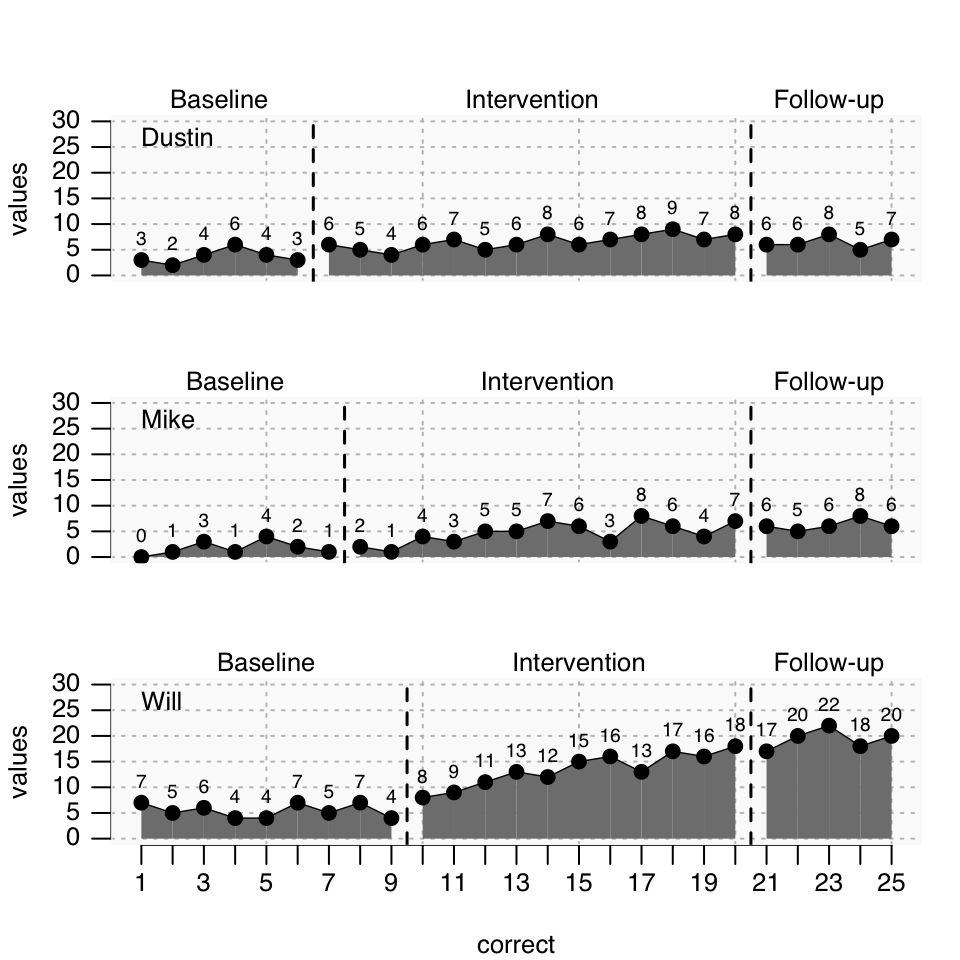
\includegraphics{scan-book_files/figure-latex/plot_strange_study-1.pdf}

Now we need some descriptive statistics:

\begin{Shaded}
\begin{Highlighting}[]
\FunctionTok{describeSC}\NormalTok{(strange\_study)}
\end{Highlighting}
\end{Shaded}

Descriptive statistics.

\begin{table}
\centering
\begin{tabular}{lccc}
\toprule
Parameter & Dustin & Mike & Will\\
\midrule
n A & 6.00 & 7.00 & 9.00\\
n B & 14.00 & 13.00 & 11.00\\
n C & 5.00 & 5.00 & 5.00\\
Missing A & 0.00 & 0.00 & 0.00\\
Missing B & 0.00 & 0.00 & 0.00\\
\addlinespace
Missing C & 0.00 & 0.00 & 0.00\\
m A & 3.67 & 1.71 & 5.44\\
m B & 6.57 & 4.69 & 13.45\\
m C & 6.40 & 6.20 & 19.40\\
md A & 3.50 & 1.00 & 5.00\\
\addlinespace
md B & 6.50 & 5.00 & 13.00\\
md C & 6.00 & 6.00 & 20.00\\
sd A & 1.37 & 1.38 & 1.33\\
sd B & 1.40 & 2.10 & 3.27\\
sd C & 1.14 & 1.10 & 1.95\\
\addlinespace
mad A & 0.74 & 1.48 & 1.48\\
mad B & 1.48 & 2.97 & 4.45\\
mad C & 1.48 & 0.00 & 2.97\\
Min A & 2.00 & 0.00 & 4.00\\
Min B & 4.00 & 1.00 & 8.00\\
\addlinespace
Min C & 5.00 & 5.00 & 17.00\\
Max A & 6.00 & 4.00 & 7.00\\
Max B & 9.00 & 8.00 & 18.00\\
Max C & 8.00 & 8.00 & 22.00\\
Trend A & 0.23 & 0.21 & -0.08\\
\addlinespace
Trend B & 0.25 & 0.36 & 0.91\\
Trend C & 0.10 & 0.30 & 0.40\\
\bottomrule
\end{tabular}
\end{table}

n = Number of measurements; Missing = Number of missing values; M = Mean; Median = Median; SD = Standard deviation; MAD = Median average deviation; Min = Minimum; Max = Maximum; Trend = Slope of dependent variable regressed on measurement-time.

Single-case data are oftentimes analyzed with overlap indices. Let us get an overview comparing phases A and B:

\begin{Shaded}
\begin{Highlighting}[]
\FunctionTok{overlap}\NormalTok{(strange\_study)}
\end{Highlighting}
\end{Shaded}

Overlap indices.Comparing phase A against phase B.

\begin{table}
\centering
\begin{tabular}{lrrr}
\toprule
  & Dustin & Mike & Will\\
\midrule
PND & 50.00 & 53.85 & 100.00\\
PEM & 100.00 & 92.31 & 100.00\\
PET & 71.43 & 61.54 & 100.00\\
NAP & 92.86 & 87.91 & 100.00\\
NAP-R & 85.71 & 75.82 & 100.00\\
\addlinespace
PAND & 90.00 & 80.00 & 100.00\\
Tau-U & 0.66 & 0.56 & 0.80\\
Base\_Tau & 0.60 & 0.55 & 0.74\\
Delta M & 2.90 & 2.98 & 8.01\\
Delta Trend & 0.02 & 0.14 & 0.99\\
\addlinespace
SMD & 2.13 & 2.16 & 6.01\\
\bottomrule
\end{tabular}
\end{table}

PND = Percentage Non-Overlapping Data; PEM = Percentage Exceeding the Median; PET = Percentage Exceeding the Trend; NAP = Nonoverlap of all pairs; NAP-R = NAP rescaled;
PAND = Percentage all nonoverlapping data;Tau U = Parker's Tau-U; Base Tau = Baseline corrected Tau; Delta M = Mean difference between phases; Delta Trend = Trend difference between phases; SMD = Standardized Mean Difference.

How do the changes hold up against the follow-up? Let us compare phases A and C:

\begin{Shaded}
\begin{Highlighting}[]
\FunctionTok{overlap}\NormalTok{(strange\_study, }\AttributeTok{phases =} \FunctionTok{c}\NormalTok{(}\StringTok{"A"}\NormalTok{, }\StringTok{"C"}\NormalTok{))}
\end{Highlighting}
\end{Shaded}

Overlap indices.Comparing phase A against phase C.

\begin{table}
\centering
\begin{tabular}{lrrr}
\toprule
  & Dustin & Mike & Will\\
\midrule
PND & 40.00 & 100.00 & 100.00\\
PEM & 100.00 & 100.00 & 100.00\\
PET & 0.00 & 60.00 & 100.00\\
NAP & 93.33 & 100.00 & 100.00\\
NAP-R & 86.67 & 100.00 & 100.00\\
\addlinespace
PAND & 81.82 & 100.00 & 100.00\\
Tau-U & 0.46 & 0.51 & 0.61\\
Base\_Tau & 0.67 & 0.76 & 0.74\\
Delta M & 2.73 & 4.49 & 13.96\\
Delta Trend & -0.13 & 0.09 & 0.48\\
\addlinespace
SMD & 2.00 & 3.25 & 10.47\\
\bottomrule
\end{tabular}
\end{table}

PND = Percentage Non-Overlapping Data; PEM = Percentage Exceeding the Median; PET = Percentage Exceeding the Trend; NAP = Nonoverlap of all pairs; NAP-R = NAP rescaled;
PAND = Percentage all nonoverlapping data;Tau U = Parker's Tau-U; Base Tau = Baseline corrected Tau; Delta M = Mean difference between phases; Delta Trend = Trend difference between phases; SMD = Standardized Mean Difference.

Finally, we conduct regression analyses for each cases with a piecewise regression model:

\begin{Shaded}
\begin{Highlighting}[]
\FunctionTok{plm}\NormalTok{(strange\_study}\SpecialCharTok{$}\NormalTok{Dustin)}
\FunctionTok{plm}\NormalTok{(strange\_study}\SpecialCharTok{$}\NormalTok{Mike)}
\FunctionTok{plm}\NormalTok{(strange\_study}\SpecialCharTok{$}\NormalTok{Will)}
\end{Highlighting}
\end{Shaded}

Piecewise-regression model for variable `values.'

\begin{table}
\centering
\begin{tabular}{lrrrrrrr}
\toprule
\multicolumn{2}{c}{ } & \multicolumn{2}{c}{CI(95\%)} & \multicolumn{4}{c}{ } \\
\cmidrule(l{3pt}r{3pt}){3-4}
Parameter & B & 2.5\% & 97.5\% & SE & t & p & Delta R²\\
\midrule
Intercept & 2.87 & 0.77 & 4.97 & 1.07 & 2.68 & <.05 & \\
Trend mt & 0.23 & -0.31 & 0.77 & 0.28 & 0.83 & .41 & .01\\
Level phase B & 0.49 & -1.58 & 2.56 & 1.06 & 0.46 & .64 & .00\\
Level phase C & -1.34 & -10.59 & 7.91 & 4.72 & -0.28 & .77 & .00\\
Slope phase B & 0.02 & -0.54 & 0.58 & 0.29 & 0.06 & .95 & .00\\
\addlinespace
Slope phase C & -0.13 & -1.02 & 0.77 & 0.46 & -0.28 & .78 & .00\\
\bottomrule
\multicolumn{8}{l}{\rule{0pt}{1em}\textit{Note: }}\\
\multicolumn{8}{l}{\rule{0pt}{1em}F(5, 19) = 7.88; p <.001; R² = 0.675; Adjusted R² = 0.589}\\
\end{tabular}
\end{table}

Piecewise-regression model for variable `values.'

\begin{table}
\centering
\begin{tabular}{lrrrrrrr}
\toprule
\multicolumn{2}{c}{ } & \multicolumn{2}{c}{CI(95\%)} & \multicolumn{4}{c}{ } \\
\cmidrule(l{3pt}r{3pt}){3-4}
Parameter & B & 2.5\% & 97.5\% & SE & t & p & Delta R²\\
\midrule
Intercept & 0.86 & -1.65 & 3.37 & 1.28 & 0.67 & .51 & \\
Trend mt & 0.21 & -0.35 & 0.78 & 0.29 & 0.75 & .46 & .01\\
Level phase B & -0.16 & -2.84 & 2.51 & 1.36 & -0.12 & .90 & .00\\
Level phase C & 0.16 & -9.41 & 9.73 & 4.88 & 0.03 & .97 & .00\\
Slope phase B & 0.14 & -0.46 & 0.75 & 0.31 & 0.46 & .64 & .00\\
\addlinespace
Slope phase C & 0.09 & -1.01 & 1.18 & 0.56 & 0.15 & .87 & .00\\
\bottomrule
\multicolumn{8}{l}{\rule{0pt}{1em}\textit{Note: }}\\
\multicolumn{8}{l}{\rule{0pt}{1em}F(5, 19) = 8.00; p <.001; R² = 0.678; Adjusted R² = 0.593}\\
\end{tabular}
\end{table}

Piecewise-regression model for variable `values.'

\begin{table}
\centering
\begin{tabular}{lrrrrrrr}
\toprule
\multicolumn{2}{c}{ } & \multicolumn{2}{c}{CI(95\%)} & \multicolumn{4}{c}{ } \\
\cmidrule(l{3pt}r{3pt}){3-4}
Parameter & B & 2.5\% & 97.5\% & SE & t & p & Delta R²\\
\midrule
Intercept & 5.86 & 3.71 & 8.01 & 1.10 & 5.35 & <.001 & \\
Trend mt & -0.08 & -0.46 & 0.30 & 0.19 & -0.43 & .67 & .00\\
Level phase B & 2.89 & 0.25 & 5.53 & 1.35 & 2.15 & <.05 & .01\\
Level phase C & 14.01 & 7.42 & 20.59 & 3.36 & 4.17 & <.001 & .05\\
Slope phase B & 0.99 & 0.52 & 1.47 & 0.24 & 4.10 & <.001 & .05\\
\addlinespace
Slope phase C & 0.48 & -0.53 & 1.49 & 0.52 & 0.94 & .35 & .00\\
\bottomrule
\multicolumn{8}{l}{\rule{0pt}{1em}\textit{Note: }}\\
\multicolumn{8}{l}{\rule{0pt}{1em}F(5, 19) = 68.16; p <.001; R² = 0.947; Adjusted R² = 0.933}\\
\end{tabular}
\end{table}

\hypertarget{some-things-about-r}{%
\chapter{Some things about R}\label{some-things-about-r}}

In this chapter you will get a brief introduction to R. If you are familiar with R you might like to go directly to the next chapter.

\hfill\break
R is a programming language optimized for statistical purposes. It was created in 1992 by Ross Ihaka and Robert Gentleman at the University of Auckland. Since then it has been developed continuously and became one of the leading statistical software programs. R is unmatched in its versatility. It is used for teaching introductory courses into statistics up to doing the most sophisticated mathematical analysis. It has become the defacto standard in many scientific disciplines from the natural to the social sciences.\\
R is completely community driven . That is, it is developed and extended by anybody who likes to participate . It comes at no costs and can be downloaded for free for all major and many minor platforms at \href{http://www.r-project.org}{www.r-project.org}. Yet, it is as reliable as other proprietary software like Mplus, STATA, SPSS etc . You can tell from my writing that is hard not to become an R-fan when you are into statistics :-)\\
R can be used in at least two ways:

\begin{enumerate}
\def\labelenumi{\arabic{enumi}.}
\tightlist
\item
  You can use it for applying data analyses. In that way it functions like most other statistical programs. You have to learn the specific syntax of R and it will compute the data analysis you need. For example \texttt{mean(x)} will return the mean of the variable \texttt{x}; \texttt{lm(y\ \textasciitilde{}\ x)} will calculate a linear regression with the criteria \texttt{y} and the predictor \texttt{x} for you or \texttt{plot(x,\ y)} will return a scatter-plot of the variables \texttt{x} and \texttt{y}.
\item
  You can use R to program new statistical procedures, or extend previous ones.
\end{enumerate}

It is the second function that is the origin of R's huge success and versatility. New statistical procedures and functions can be published to be used for everyone in so called packages. A package usually contains several functions, help files and example data-sets. Hundreds of such packages are available to help in all kinds of specialized analyses. The basic installation of R comes with a large variety of packages per installed. New packages can most of the times be easily installed from within R. Admittedly, if you must have the latest developmental version of a new package installation sometimes can get a bit more complex. But with a bit of help and persistence it is not to difficult to accomplish.

The book at hand describes the use of such an additional package named \emph{scan} providing specialized functions for single-case analyses. \emph{scan} comes in two versions: A ``stable'' version and a developmental version. Both versions can be installed directly from within R. The stable version is much older and only provides a limited functionality. Therefore, I will refer to the developmental version in this book.

\hypertarget{basic-r}{%
\section{Basic R}\label{basic-r}}

\emph{R} is a script language. That is, you type in text and let R execute the commands you wrote down. Either you work in a \emph{console} or a \emph{textfile}. In a \emph{console} the command will be executed every time you press the RETURN-key. In a \emph{textfile} you type down your code, mark the part you like to be executed, and run that code (with a click or a certain key). The latter text files can be saved and reused for later R sessions. Therefore, usually you will work in a text file.

A value is assigned to a variable with the \texttt{\textless{}-} operator. Which should be read as an arrow rather than a less sign and a minus sign. A \texttt{\#} is followed by a comment to make your code more understandable. So, what follows a \texttt{\#} is not interpreted by R. A vector is a chain of several values. With a vector you could describe the values of a measurement series. The \texttt{c} function is used to build a vector (e.g., \texttt{c(1,\ 2,\ 3,\ 4)}). If you like to see the content of a variable you could use the \texttt{print} function. \texttt{print(x)} will display the content of the variable \texttt{x}. A shortcut for this is just to type variable name (and press return) \texttt{x}.

\begin{Shaded}
\begin{Highlighting}[]
\CommentTok{\# x is assigned the value 10:}
\NormalTok{x }\OtherTok{\textless{}{-}} \DecValTok{10}

\CommentTok{\# See what\textquotesingle{}s inside of x:}
\NormalTok{x}
\end{Highlighting}
\end{Shaded}

\begin{verbatim}
[1] 10
\end{verbatim}

\begin{Shaded}
\begin{Highlighting}[]
\CommentTok{\# x is assigned a vector with three values:}
\NormalTok{x }\OtherTok{\textless{}{-}} \FunctionTok{c}\NormalTok{(}\DecValTok{10}\NormalTok{, }\DecValTok{11}\NormalTok{, }\DecValTok{15}\NormalTok{)}

\CommentTok{\# ... and display the content of x:}
\NormalTok{x}
\end{Highlighting}
\end{Shaded}

\begin{verbatim}
[1] 10 11 15
\end{verbatim}

Two important concepts in \textbf{R} are \emph{functions} and \emph{arguments}. A \emph{function} is the name for a procedure that does something with the \emph{arguments} that are provided by you. For example, the function \texttt{mean} calculated the mean. \texttt{mean} has an argument \texttt{x} which ``expects'' that you provide a vector (a series of values) from which it will calculate the mean. \texttt{mean(\ x\ =\ c(1,\ 3,\ 5)\ )} will compute the mean of the values 1, 3, and 5 and return the result 3. Some \emph{functions} can take several arguments. \texttt{mean} for example also takes the argument \texttt{trim}. For calculating a trimmed mean. \texttt{mean(\ x\ =\ c(1,\ 1,\ 3,\ 3,\ 5,\ 6,\ 7,\ 8,\ 9,\ 9),\ trim\ =\ 0.1)} will calculate the 10\% trimmed mean of the provided values. The name of the first argument could be dropped. That is, \texttt{mean(\ c(1,\ 3,\ 5)\ )} will be interpreted by \textbf{R} as \texttt{mean(\ x\ =\ c(1,\ 3,\ 5)\ )}. You could also provide a variable to an argument.

\begin{Shaded}
\begin{Highlighting}[]
\NormalTok{values }\OtherTok{\textless{}{-}} \FunctionTok{c}\NormalTok{(}\DecValTok{1}\NormalTok{, }\DecValTok{4}\NormalTok{, }\DecValTok{5}\NormalTok{, }\DecValTok{6}\NormalTok{, }\DecValTok{3}\NormalTok{, }\DecValTok{7}\NormalTok{, }\DecValTok{7}\NormalTok{, }\DecValTok{5}\NormalTok{)}
\FunctionTok{mean}\NormalTok{(}\AttributeTok{x =}\NormalTok{ values)}
\end{Highlighting}
\end{Shaded}

\begin{verbatim}
[1] 4.75
\end{verbatim}

\begin{Shaded}
\begin{Highlighting}[]
\CommentTok{\# or shorter:}
\FunctionTok{mean}\NormalTok{(values)}
\end{Highlighting}
\end{Shaded}

\begin{verbatim}
[1] 4.75
\end{verbatim}

The return value of a function can be assigned to a new variable instead:

\begin{Shaded}
\begin{Highlighting}[]
\NormalTok{y }\OtherTok{\textless{}{-}} \FunctionTok{c}\NormalTok{(}\DecValTok{1}\NormalTok{, }\DecValTok{4}\NormalTok{, }\DecValTok{5}\NormalTok{, }\DecValTok{6}\NormalTok{, }\DecValTok{3}\NormalTok{, }\DecValTok{7}\NormalTok{, }\DecValTok{7}\NormalTok{, }\DecValTok{5}\NormalTok{)}
\NormalTok{res }\OtherTok{\textless{}{-}} \FunctionTok{mean}\NormalTok{(y)}
\CommentTok{\#now res contains the mean of y:}
\NormalTok{res}
\end{Highlighting}
\end{Shaded}

\begin{verbatim}
[1] 4.75
\end{verbatim}

Every function in R has a help page written by the programmers. You can retrieve these pages with the \texttt{help} function or the short cut \texttt{?}. \texttt{help("mean")} will display the help page for the \texttt{mean} function. The quotation marks are necessary here because you do not provide a variable with the name \emph{mean} but a word `mean.' The shortcut works \texttt{?mean}. A bit confusingly, you do not need the quotation marks here.

\hypertarget{managing-single-case-data}{%
\chapter{Managing single-case data}\label{managing-single-case-data}}

\hypertarget{a-single-case-data-frame}{%
\section{\texorpdfstring{A \textbf{\emph{single-case data frame}}}{A single-case data frame}}\label{a-single-case-data-frame}}

Scan provides its own data-class for encoding single-case data: the \emph{single-case data frame} (short \emph{scdf}). An \emph{scdf} is an object that contains one or multiple single-case data sets and is optimized for managing and displaying these data. Think of an scdf as a file including a separate datasheet for each single case. Each datasheet is made up of at least three variables: The measured \textbf{values}, the \textbf{phase} identifier for each measured value, and the measurement time (\textbf{mt}) of each measure. Optionally, scdfs could include further variables for each single-case (e.g., control variables), and also a name for each case.

\begin{rmdnote}
Technically, an scdf object is a list containing data frames. It is of
the class \texttt{c("scdf","list")}. Additionally, an \emph{scdf}
entails an attribute \texttt{scdf} with a list with further attributes.
\texttt{var.values}, \texttt{var.phase}, and \texttt{var.mt} contain the
names of the \texttt{values}, \texttt{phase}, and the
\texttt{measurement\ time} variable. By default, these names are set to
\texttt{values}, \texttt{phase}, and \texttt{mt}.
\end{rmdnote}

Several functions are available for creating, transforming, merging, and importing/exporting \emph{scdfs}.

\hypertarget{creating-scdfs}{%
\section{Creating scdfs}\label{creating-scdfs}}

The \texttt{scdf} function is the basic tool for creating a single-case data frame. Basically, you have to provide the measurement \emph{values} and the \emph{phase} structure and a scdf object is build. There are three different ways of defining the phase structure. First, defining the beginning of the B-phase with the \texttt{B.start} argument, second, defining a design with the \texttt{phase.design} argument and third, setting parameters in a named vector of the dependent variable.

\begin{Shaded}
\begin{Highlighting}[]
\DocumentationTok{\#\#\# Three ways to code the same scdf}
\FunctionTok{scdf}\NormalTok{(}\AttributeTok{values =} \FunctionTok{c}\NormalTok{(}\AttributeTok{A =} \DecValTok{2}\NormalTok{,}\DecValTok{2}\NormalTok{,}\DecValTok{4}\NormalTok{,}\DecValTok{5}\NormalTok{, }\AttributeTok{B =} \DecValTok{8}\NormalTok{,}\DecValTok{7}\NormalTok{,}\DecValTok{6}\NormalTok{,}\DecValTok{9}\NormalTok{,}\DecValTok{8}\NormalTok{,}\DecValTok{7}\NormalTok{))}
\FunctionTok{scdf}\NormalTok{(}\AttributeTok{values =} \FunctionTok{c}\NormalTok{(}\DecValTok{2}\NormalTok{,}\DecValTok{2}\NormalTok{,}\DecValTok{4}\NormalTok{,}\DecValTok{5}\NormalTok{,}\DecValTok{8}\NormalTok{,}\DecValTok{7}\NormalTok{,}\DecValTok{6}\NormalTok{,}\DecValTok{9}\NormalTok{,}\DecValTok{8}\NormalTok{,}\DecValTok{7}\NormalTok{), }\AttributeTok{B.start =} \DecValTok{5}\NormalTok{)}
\FunctionTok{scdf}\NormalTok{(}\AttributeTok{values =} \FunctionTok{c}\NormalTok{(}\DecValTok{2}\NormalTok{,}\DecValTok{2}\NormalTok{,}\DecValTok{4}\NormalTok{,}\DecValTok{5}\NormalTok{,}\DecValTok{8}\NormalTok{,}\DecValTok{7}\NormalTok{,}\DecValTok{6}\NormalTok{,}\DecValTok{9}\NormalTok{,}\DecValTok{8}\NormalTok{,}\DecValTok{7}\NormalTok{), }\AttributeTok{phase.design =} \FunctionTok{c}\NormalTok{(}\AttributeTok{A =} \DecValTok{4}\NormalTok{, }\AttributeTok{B =} \DecValTok{6}\NormalTok{))}
\end{Highlighting}
\end{Shaded}

The \texttt{B.start} argument is only applicable when the single-case consists of a single A-phase followed by a B-phase. It is a remnant from the time when \texttt{scan} could only handle sign-case designs with two phases. The number assigned to \texttt{B.start} indicates the measurement-time as defined in the \texttt{mt} argument. That is, assume a vector for the measurement times \texttt{mt\ =\ c(1,3,7,10,15,17,18,20)} and \texttt{B.start\ =\ 15} then the first measurement of the B-phase will start with the fifth measurement at which \emph{mt} = 15.\\
The \texttt{phase.design} argument is a named vector with the name and length of each phase. The phase names can be set arbitrary, although I recommend to use capital letters (A, B, C, \ldots) for each phase followed by, when indicated, a number if the phases repeat (A1, B1, A2, B2, \ldots). Although it is possible to give the same name to more than one phase (A, B, A, B) this might lead to some confusion and errors when coding analyzes with \emph{scan}.\\
When the vector of the dependent variable includes named values, a phase.design structure is created automatically. Each named value sets the beginning of a new phase. For example \texttt{c(A\ =\ 3,2,4,\ B\ =\ 5,4,3,\ C\ =\ 6,7,6,5)} will create an ABC-phase design with 3, 3, and 4 values per phase.\\
Use only one of the three methods at a time and I recommend to use the \texttt{phase.design} argument or the named vector method as they are the most versatile.\\
If no measurement times are given, scdf automatically adds them numbered sequentially 1, 2, 3, \ldots, \emph{N} where \emph{N} is the number of measurements. in some circumstances it might be useful to define individual measurement times for each measurement. For example, if you want to include the days since the beginning of the study as time intervals between measurements are widely varying you might get more valid results this way when analyzing the data in a regression approach.

\begin{Shaded}
\begin{Highlighting}[]
\CommentTok{\# example of a more complex design }
\FunctionTok{scdf}\NormalTok{(}
  \AttributeTok{values =} \FunctionTok{c}\NormalTok{(}\DecValTok{2}\NormalTok{,}\DecValTok{2}\NormalTok{,}\DecValTok{4}\NormalTok{,}\DecValTok{5}\NormalTok{, }\DecValTok{8}\NormalTok{,}\DecValTok{7}\NormalTok{,}\DecValTok{6}\NormalTok{,}\DecValTok{9}\NormalTok{,}\DecValTok{8}\NormalTok{,}\DecValTok{7}\NormalTok{, }\DecValTok{12}\NormalTok{,}\DecValTok{11}\NormalTok{,}\DecValTok{13}\NormalTok{), }
  \AttributeTok{mt =} \FunctionTok{c}\NormalTok{(}\DecValTok{1}\NormalTok{,}\DecValTok{2}\NormalTok{,}\DecValTok{3}\NormalTok{,}\DecValTok{6}\NormalTok{, }\DecValTok{8}\NormalTok{,}\DecValTok{9}\NormalTok{,}\DecValTok{11}\NormalTok{,}\DecValTok{12}\NormalTok{,}\DecValTok{16}\NormalTok{,}\DecValTok{18}\NormalTok{, }\DecValTok{27}\NormalTok{,}\DecValTok{28}\NormalTok{,}\DecValTok{29}\NormalTok{),}
  \AttributeTok{phase.design =} \FunctionTok{c}\NormalTok{(}\AttributeTok{A =} \DecValTok{4}\NormalTok{, }\AttributeTok{B =} \DecValTok{6}\NormalTok{, }\AttributeTok{C =} \DecValTok{3}\NormalTok{)}
\NormalTok{)}
\end{Highlighting}
\end{Shaded}

\begin{verbatim}
#A single-case data frame with one case

 Case1: values mt phase
             2  1     A
             2  2     A
             4  3     A
             5  6     A
             8  8     B
             7  9     B
             6 11     B
             9 12     B
             8 16     B
             7 18     B
            12 27     C
            11 28     C
            13 29     C
\end{verbatim}

Missing values could be coded using \texttt{NA}.

\begin{Shaded}
\begin{Highlighting}[]
\FunctionTok{scdf}\NormalTok{(}\AttributeTok{values =} \FunctionTok{c}\NormalTok{(}\AttributeTok{A =} \DecValTok{2}\NormalTok{,}\DecValTok{2}\NormalTok{,}\ConstantTok{NA}\NormalTok{,}\DecValTok{5}\NormalTok{, }\AttributeTok{B =} \DecValTok{8}\NormalTok{,}\DecValTok{7}\NormalTok{,}\DecValTok{6}\NormalTok{,}\DecValTok{9}\NormalTok{,}\ConstantTok{NA}\NormalTok{,}\DecValTok{7}\NormalTok{))}
\end{Highlighting}
\end{Shaded}

More variables are implemented by adding new variable names with a vector containing the values. Please be aware that a new variable must never have the same name as one of the arguments of the function (i.e.~B.start, phase.design, name, dvar, pvar, mvar).

\begin{Shaded}
\begin{Highlighting}[]
\FunctionTok{scdf}\NormalTok{(}
  \AttributeTok{values =} \FunctionTok{c}\NormalTok{(}\AttributeTok{A =} \DecValTok{2}\NormalTok{,}\DecValTok{2}\NormalTok{,}\DecValTok{3}\NormalTok{,}\DecValTok{5}\NormalTok{, }\AttributeTok{B =} \DecValTok{8}\NormalTok{,}\DecValTok{7}\NormalTok{,}\DecValTok{6}\NormalTok{,}\DecValTok{9}\NormalTok{,}\DecValTok{7}\NormalTok{,}\DecValTok{7}\NormalTok{), }
  \AttributeTok{teacher =} \FunctionTok{c}\NormalTok{(}\DecValTok{0}\NormalTok{,}\DecValTok{0}\NormalTok{,}\DecValTok{1}\NormalTok{,}\DecValTok{1}\NormalTok{,}\DecValTok{0}\NormalTok{,}\DecValTok{1}\NormalTok{,}\DecValTok{1}\NormalTok{,}\DecValTok{1}\NormalTok{,}\DecValTok{0}\NormalTok{,}\DecValTok{1}\NormalTok{), }
  \AttributeTok{hour =} \FunctionTok{c}\NormalTok{(}\DecValTok{2}\NormalTok{,}\DecValTok{3}\NormalTok{,}\DecValTok{4}\NormalTok{,}\DecValTok{3}\NormalTok{,}\DecValTok{3}\NormalTok{,}\DecValTok{1}\NormalTok{,}\DecValTok{6}\NormalTok{,}\DecValTok{5}\NormalTok{,}\DecValTok{2}\NormalTok{,}\DecValTok{2}\NormalTok{)}
\NormalTok{)}
\end{Highlighting}
\end{Shaded}

\begin{verbatim}
#A single-case data frame with one case

 Case1: values teacher hour mt phase
             2       0    2  1     A
             2       0    3  2     A
             3       1    4  3     A
             5       1    3  4     A
             8       0    3  5     B
             7       1    1  6     B
             6       1    6  7     B
             9       1    5  8     B
             7       0    2  9     B
             7       1    2 10     B
\end{verbatim}

Table \ref{tab:table-scdf} shows a complete list of arguments that could be passed to the function.

\begin{table}

\caption{\label{tab:table-scdf}Arguments of the scdf function}
\centering
\begin{tabular}[t]{>{\raggedright\arraybackslash}p{15em}>{\raggedright\arraybackslash}p{30em}}
\toprule
Argument & What it does ...\\
\midrule
\textbf{values} & The default vector with values for the dependent variable. It can be changed with the dvar argument.\\
\textbf{phase} & Usually, this variable is not defined manually and will be created by the function. It is the default vector with values for the phase variable. It can be changed with the pvar argument.\\
\textbf{mt} & The default vector with values for the measurement-time variable. It can be changed with the mvar argument.\\
\textbf{phase.design} & A vector defining the length and label of each phase.\\
\textbf{B.start} & The first measurement of phase B (simple coding if design is strictly AB).\\
\addlinespace
\textbf{name} & A name for the case.\\
\textbf{dvar} & The name of the dependent variable. By default this is 'values'.\\
\textbf{pvar} & The name of the variable containing the phase information. By default this is 'phase'.\\
\textbf{mvar} & The name of the variable with the measurement-time. The default is 'mt'.\\
\textbf{...} & Any number of variables with a vector asigned to them.\\
\bottomrule
\end{tabular}
\end{table}

If you want to create a data-set comprising several single-cases the easiest way is to first create an scdf for each case and then join them into a new scdf with the \texttt{c} command:

\begin{Shaded}
\begin{Highlighting}[]
\NormalTok{case1 }\OtherTok{\textless{}{-}} \FunctionTok{scdf}\NormalTok{(}
  \AttributeTok{values =} \FunctionTok{c}\NormalTok{(}\AttributeTok{A =} \DecValTok{5}\NormalTok{, }\DecValTok{7}\NormalTok{, }\DecValTok{10}\NormalTok{, }\DecValTok{5}\NormalTok{, }\DecValTok{12}\NormalTok{, }\AttributeTok{B =} \DecValTok{7}\NormalTok{, }\DecValTok{10}\NormalTok{, }\DecValTok{18}\NormalTok{, }\DecValTok{15}\NormalTok{, }\DecValTok{14}\NormalTok{, }\DecValTok{19}\NormalTok{), }
  \AttributeTok{name =} \StringTok{"Charlotte"}
\NormalTok{)}
\NormalTok{case2 }\OtherTok{\textless{}{-}} \FunctionTok{scdf}\NormalTok{(}
  \AttributeTok{values =} \FunctionTok{c}\NormalTok{(}\AttributeTok{A =} \DecValTok{3}\NormalTok{, }\DecValTok{4}\NormalTok{, }\DecValTok{3}\NormalTok{, }\DecValTok{5}\NormalTok{, }\AttributeTok{B =} \DecValTok{7}\NormalTok{, }\DecValTok{4}\NormalTok{, }\DecValTok{7}\NormalTok{, }\DecValTok{9}\NormalTok{, }\DecValTok{8}\NormalTok{, }\DecValTok{10}\NormalTok{, }\DecValTok{12}\NormalTok{), }
  \AttributeTok{name =} \StringTok{"Theresa"}
\NormalTok{)}
\NormalTok{case3 }\OtherTok{\textless{}{-}} \FunctionTok{scdf}\NormalTok{(}
  \AttributeTok{values =} \FunctionTok{c}\NormalTok{(}\AttributeTok{A =} \DecValTok{9}\NormalTok{, }\DecValTok{8}\NormalTok{, }\DecValTok{8}\NormalTok{, }\DecValTok{7}\NormalTok{, }\DecValTok{5}\NormalTok{, }\DecValTok{7}\NormalTok{, }\AttributeTok{B =} \DecValTok{6}\NormalTok{, }\DecValTok{14}\NormalTok{, }\DecValTok{15}\NormalTok{, }\DecValTok{12}\NormalTok{, }\DecValTok{16}\NormalTok{), }
  \AttributeTok{name =} \StringTok{"Antonia"}
\NormalTok{)}
\NormalTok{mbd }\OtherTok{\textless{}{-}} \FunctionTok{c}\NormalTok{(case1, case2, case3)}
\end{Highlighting}
\end{Shaded}

If you like to use other than the default variable names (``values,'' ``phase,'' and ``mt'') you could define these with the \texttt{dvar} (for the dependent variable), \texttt{pvar} (the variable indicating the phase), and \texttt{mvar} (the measurement-time variable) arguments.

\begin{Shaded}
\begin{Highlighting}[]
\CommentTok{\# Example: Using a different name for the dependent variable}
\NormalTok{case }\OtherTok{\textless{}{-}} \FunctionTok{scdf}\NormalTok{(}
  \AttributeTok{score =} \FunctionTok{c}\NormalTok{(}\AttributeTok{A =} \DecValTok{5}\NormalTok{, }\DecValTok{7}\NormalTok{, }\DecValTok{10}\NormalTok{, }\DecValTok{5}\NormalTok{, }\DecValTok{12}\NormalTok{, }\AttributeTok{B =} \DecValTok{7}\NormalTok{, }\DecValTok{10}\NormalTok{, }\DecValTok{18}\NormalTok{, }\DecValTok{15}\NormalTok{, }\DecValTok{14}\NormalTok{, }\DecValTok{19}\NormalTok{), }
  \AttributeTok{dvar =} \StringTok{"score"}
\NormalTok{)}

\CommentTok{\# Example: Using new names for the dependent and the phase variables}
\NormalTok{case }\OtherTok{\textless{}{-}} \FunctionTok{scdf}\NormalTok{(}
  \AttributeTok{score =} \FunctionTok{c}\NormalTok{(}\AttributeTok{A =} \DecValTok{3}\NormalTok{, }\DecValTok{4}\NormalTok{, }\DecValTok{3}\NormalTok{, }\DecValTok{5}\NormalTok{, }\AttributeTok{B =} \DecValTok{7}\NormalTok{, }\DecValTok{4}\NormalTok{, }\DecValTok{7}\NormalTok{, }\DecValTok{9}\NormalTok{, }\DecValTok{8}\NormalTok{, }\DecValTok{10}\NormalTok{, }\DecValTok{12}\NormalTok{), }
  \AttributeTok{dvar =} \StringTok{"score"}\NormalTok{, }\AttributeTok{pvar =} \StringTok{"section"}
\NormalTok{)}

\CommentTok{\# Example: Using new names for dependent, phase, and measurement{-}time variables}
\NormalTok{case }\OtherTok{\textless{}{-}} \FunctionTok{scdf}\NormalTok{(}
  \AttributeTok{score =} \FunctionTok{c}\NormalTok{(}\AttributeTok{A =} \DecValTok{9}\NormalTok{, }\DecValTok{8}\NormalTok{, }\DecValTok{8}\NormalTok{, }\DecValTok{7}\NormalTok{, }\DecValTok{5}\NormalTok{, }\DecValTok{7}\NormalTok{, }\AttributeTok{B =} \DecValTok{6}\NormalTok{, }\DecValTok{14}\NormalTok{, }\DecValTok{15}\NormalTok{, }\DecValTok{12}\NormalTok{, }\DecValTok{16}\NormalTok{), }
  \AttributeTok{name =} \StringTok{"Antonia"}\NormalTok{, }\AttributeTok{dvar =} \StringTok{"score"}\NormalTok{, }\AttributeTok{pvar =} \StringTok{"section"}\NormalTok{, }\AttributeTok{mvar =} \StringTok{"day"}
\NormalTok{)}

\FunctionTok{summary}\NormalTok{(case)}
\end{Highlighting}
\end{Shaded}

\begin{verbatim}
#A single-case data frame with one case

        Measurements Design
Antonia           11    A B

Variable names:
score <dependent variable>
day <measurement-time variable>
section <phase variable>
\end{verbatim}

\hypertarget{saving-and-reading-single-case-data-frames}{%
\section{\texorpdfstring{Saving and reading \emph{single-case data frames}}{Saving and reading single-case data frames}}\label{saving-and-reading-single-case-data-frames}}

Usually, it is not needed to save an scdf to a separate file on your computer. In most of the cases you could keep the coding of the \emph{scdf} as described above and rerun it every time that you are working with your data. But sometimes it is more convenient to separately save the data to a file for later use or to send them to a colleague.\\
The simplest way is to use the base \emph{R} functions \texttt{saveRDS} and \texttt{readRDS} for this purpose. \texttt{saveRDS} takes at least two arguments: the first is the object you like to save and the second is a file name for the resulting file. If you have an \emph{scdf} with the name \texttt{study1} the line \texttt{saveRDS(study1,\ "study1.rds")} will save the \emph{scdf} to your drive. You could later read this file with \texttt{study1\ \textless{}-\ readRDS("study1.rds")}. \texttt{getwd()} will return the current active folder that you are working in.

\hypertarget{import-and-export-single-case-data-frames}{%
\section{\texorpdfstring{Import and export \emph{single-case data frames}}{Import and export single-case data frames}}\label{import-and-export-single-case-data-frames}}

When you are working with other programs besides \textbf{R} you need to export and import the \emph{scdf} into a common file format. \texttt{readSC} imports a comma-separated-variable (\emph{csv}) file and converts it into an \emph{scdf} object. By default, the csv-file has to contain the columns \emph{case}, \emph{phase}, and \emph{values}. Optionally, a further column named \emph{mt} could be provided. The csv file should be build up like this:

\begin{figure}
\centering
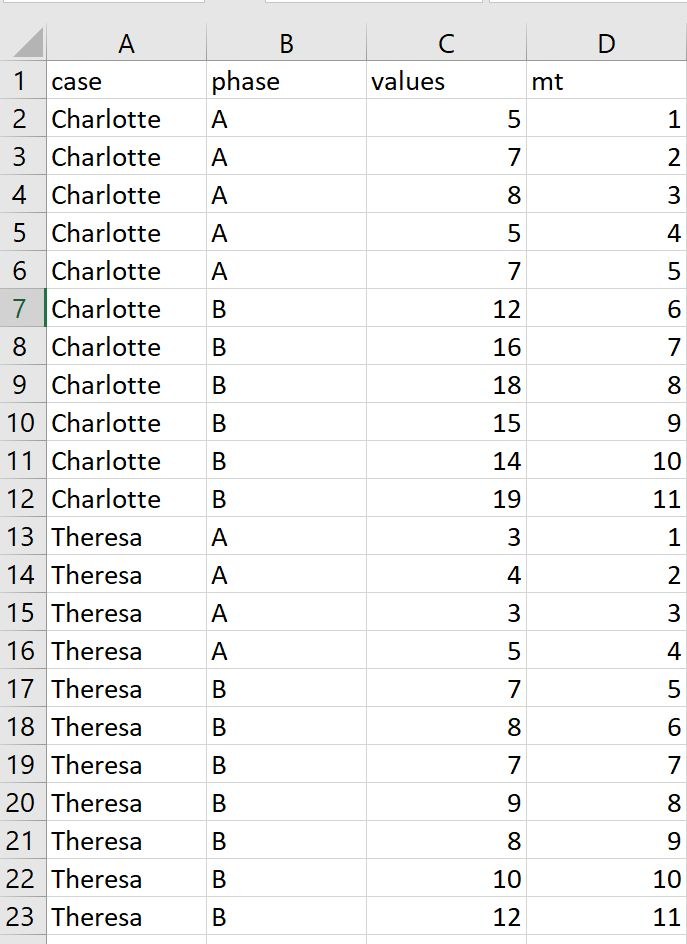
\includegraphics[width=3.125in,height=\textheight]{images/readSC.jpg}
\caption{How to format a single-case file in a spreadsheet program for importing into scan}
\end{figure}

In case your variables names differ from the standard (i.e.~``case,'' ``values,'' ``phase,'' and ``mt'' ), you could set additional arguments to fit your file. \texttt{readSC("example.csv",\ cvar\ =\ "name",\ dvar\ =\ "wellbeing",\ pvar\ =\ "intervention",\ mvar\ =\ "time")} for example will set the variables attributes of the resulting scdf. Cases will be split by the variable \texttt{"name"}, \texttt{"wellbeing"} is set as the dependent variable (default is \emph{values}), phase information are in the variable \texttt{"intervention"}, and measurement times in the variable \texttt{"time"}. You could also reassign the phase names within the phase variable by setting the argument \texttt{phase.names}. Assume for example your file contains the values 0 and 1 to identify the two phases I recommend to set them to ``A'' and ``B'' with \texttt{readSC("example.csv",\ phase.names\ =\ c("A",\ "B"))}.

\begin{Shaded}
\begin{Highlighting}[]
\NormalTok{dat }\OtherTok{\textless{}{-}} \FunctionTok{readSC.excel}\NormalTok{(}
  \StringTok{"example2.xlsx"}\NormalTok{, }\AttributeTok{cvar =} \StringTok{"name"}\NormalTok{, }\AttributeTok{pvar =} \StringTok{"intervention"}\NormalTok{, }
  \AttributeTok{dvar =} \StringTok{"wellbeing"}\NormalTok{, }\AttributeTok{mvar =} \StringTok{"time"}\NormalTok{, }\AttributeTok{phase.names =} \FunctionTok{c}\NormalTok{(}\StringTok{"A"}\NormalTok{,}\StringTok{"B"}\NormalTok{)}
\NormalTok{)}
\end{Highlighting}
\end{Shaded}

\begin{verbatim}
Imported 20 cases.
\end{verbatim}

\begin{Shaded}
\begin{Highlighting}[]
\FunctionTok{summary}\NormalTok{(dat)}
\end{Highlighting}
\end{Shaded}

\begin{verbatim}
#A single-case data frame with 20 cases

         Measurements Design
Charles            20    A B
Kolten             20    A B
Annika             20    A B
Kaysen             20    A B
Urijah             20    A B
Leila              20    A B
Leia               20    A B
Aleigha            20    A B
Greta              20    A B
Alijah             20    A B
Ricardo            20    A B
Dallas             20    A B
Edith              20    A B
Braylee            20    A B
Giovanni           20    A B
Ismael             20    A B
Grady              20    A B
Raina              20    A B
Cambria            20    A B
Lincoln            20    A B

Variable names:
intervention <phase variable>
wellbeing <dependent variable>
time <measurement-time variable>
age
gender
gym
\end{verbatim}

For some reasons, computer systems with a German (and some other) language setups export csv-files by default with a comma as a decimal point and a semicolon as a separator between values. In these cases you have to set two extra arguments to import the data:

\texttt{readSC("example.csv",\ dec\ =\ ",",\ sep\ =\ ";")}

\texttt{readSC.excel} allows for directly importing \emph{Microsoft Excel} \texttt{.xlsx} or \texttt{.xls} files. You need to have the library \texttt{readxl} installed in your R setup for this to work.

\texttt{writeSC} exports an scdf object as a comma-separated-variables file (\emph{csv}) which can be imported into any other software for data analyses (MS OFFICE, Libre Office etc.). The scdf object is converted into a single data frame with a \emph{case} variable identifying the rows for each subject. The first argument of the command identifies the scdf to be exported and the second argument (\texttt{file}) the name of the resulting csv-file. If no file argument is provided, a dialog box is opened to choose a file interactively. By default, writeSC exports into a standard csv-format with a dot as the decimal point and a comma for separating variables. If your system expects a comma instead of a point for decimal numbers you may use the \texttt{dec} and the \texttt{sep} arguments. For example, \texttt{writeSC(example,\ file\ =\ "example.csv",\ dec\ =\ ",",\ sep\ =\ ";")} exports a csv variation usually used for example in Germany.

\hypertarget{displaying-and-manipulating-scdf-files}{%
\section{Displaying and manipulating scdf-files}\label{displaying-and-manipulating-scdf-files}}

\emph{scdf} are displayed by just typing the name of the object.

\begin{Shaded}
\begin{Highlighting}[]
\CommentTok{\#Beretvas2008 is an example scdf included in scan}
\NormalTok{Beretvas2008}
\end{Highlighting}
\end{Shaded}

\begin{verbatim}
#A single-case data frame with one case

 Case1: values mt phase
           0.7  1     A
           1.6  2     A
           1.4  3     A
           1.6  4     A
           1.9  5     A
           1.2  6     A
           1.3  7     A
           1.6  8     A
            10  9     B
          10.8 10     B
          11.9 11     B
            11 12     B
            13 13     B
          12.7 14     B
            14 15     B
\end{verbatim}

The \texttt{print} command allows for specifying the output. Some possible arguments are \texttt{cases} (the number of cases to be displayed; Three by default), \texttt{rows} (the maximum number of rows to be displayed; Fifteen by default), and \texttt{digits} (number of digits). \texttt{cases\ =\ \textquotesingle{}all\textquotesingle{}} and \texttt{rows\ =\ \textquotesingle{}all\textquotesingle{}} prints all cases and rows.

\begin{Shaded}
\begin{Highlighting}[]
\CommentTok{\#Huber2014 is an example scdf included in scan}
\FunctionTok{print}\NormalTok{(Huber2014, }\AttributeTok{cases =} \DecValTok{2}\NormalTok{, }\AttributeTok{rows =} \DecValTok{10}\NormalTok{)}
\end{Highlighting}
\end{Shaded}

\begin{verbatim}
#A single-case data frame with 4 cases

 Adam: mt compliance phase | Berta: mt compliance phase |
        1         25     A |         1         25     A |
        2       20.8     A |         2       20.8     A |
        3       39.6     A |         3       39.6     A |
        4         75     A |         4         75     A |
        5         45     A |         5         45     A |
        6       39.6     A |         6       14.6     A |
        7       54.2     A |         7       45.8     A |
        8         50     A |         8       33.3     A |
        9       28.1     A |         9       31.3     A |
       10         40     A |        10       32.5     A |
# ... up to 66 more rows
#  2 more cases
\end{verbatim}

The argument \texttt{long\ =\ TRUE} prints each case one after the other instead side by side (e.g., \texttt{print(exampleAB,\ long\ =\ TRUE)}).

\texttt{summary()} gives a very concise overview of the \emph{scdf}

\begin{Shaded}
\begin{Highlighting}[]
\FunctionTok{summary}\NormalTok{(Huber2014)}
\end{Highlighting}
\end{Shaded}

\begin{verbatim}
#A single-case data frame with 4 cases

          Measurements Design
Adam                37    A B
Berta               29    A B
Christian           76    A B
David               76    A B

Variable names:
mt <measurement-time variable>
compliance <dependent variable>
phase <phase variable>


Note:  Behavioral data (compliance in percent).
Author of data:  Christian Huber 
\end{verbatim}

You can extract one or more single-cases from an \emph{scdf} with multiple cases in two ways. If the case has a name, you can address it with the \texttt{\$} operator.

\begin{Shaded}
\begin{Highlighting}[]
\NormalTok{Huber2014}\SpecialCharTok{$}\NormalTok{David}
\end{Highlighting}
\end{Shaded}

or you can use squared brackets

\begin{Shaded}
\begin{Highlighting}[]
\NormalTok{Huber2014[}\DecValTok{1}\NormalTok{] }\CommentTok{\#extracts case 1}
\NormalTok{Huber2014[}\DecValTok{2}\SpecialCharTok{:}\DecValTok{3}\NormalTok{] }\CommentTok{\#extracts cases 2 and 3}
\end{Highlighting}
\end{Shaded}

\begin{Shaded}
\begin{Highlighting}[]
\NormalTok{new.huber2014 }\OtherTok{\textless{}{-}}\NormalTok{ Huber2014[}\FunctionTok{c}\NormalTok{(}\DecValTok{1}\NormalTok{, }\DecValTok{4}\NormalTok{)] }\CommentTok{\#extracts cases 1 and 4}
\FunctionTok{print}\NormalTok{(new.huber2014)}
\end{Highlighting}
\end{Shaded}

\begin{verbatim}
#A single-case data frame with 2 cases

 Adam: mt compliance phase | David: mt compliance phase |
        1         25     A |         1       65.6     A |
        2       20.8     A |         2       37.5     A |
        3       39.6     A |         3       58.3     A |
        4         75     A |         4       72.9     A |
        5         45     A |         5       33.3     A |
        6       39.6     A |         6       59.4     A |
        7       54.2     A |         7       77.1     A |
        8         50     A |         8       54.2     A |
        9       28.1     A |         9       68.8     A |
       10         40     A |        10       43.8     A |
       11       52.1     B |        11       62.5     B |
       12       31.3     B |        12       64.6     B |
       13       15.6     B |        13       60.4     B |
       14       29.2     B |        14       81.3     B |
       15       43.8     B |        15       79.2     B |
# ... up to 61 more rows
\end{verbatim}

\hypertarget{creating-a-single-case-data-plot}{%
\chapter{Creating a single-case data plot}\label{creating-a-single-case-data-plot}}

Plotting the data is a first important approach of analyzing. After you build an \emph{scdf} the \texttt{plot} command helps to visualize the data. When the \texttt{scdf} includes more than one case a multiple baseline figure is provided. Various arguments can be set to customize the appearance of the plot. Table \ref{tab:table-plot-arguments} gives an overview of all available arguments.\\
Labels of the axes and for the phases can be changed with the \texttt{xlab}, \texttt{ylab}, and the \texttt{phase.names} arguments. The x- and y-scaling of the graphs are by default calculated as the minimum and the maximum of all included single cases. The \texttt{xlim} and the \texttt{ylim} argument are used to set specific values. The argument takes a vector of two numbers. The first for the lower and the second for the upper limit of the scale. In case of multiple single cases an \texttt{NA} sets the individual minimum or maximum for each case. Assume for example the study contains three single cases \texttt{ylim\ =\ c(0,\ NA)} will set the lower limit for all three single cases to \texttt{0} and the upper limit individually at the maximum of each case.

\begin{table}

\caption{\label{tab:table-plot-arguments}Arguments of the plot function}
\centering
\begin{tabular}[t]{>{\raggedright\arraybackslash}p{15em}>{\raggedright\arraybackslash}p{30em}}
\toprule
Argument & What it does ...\\
\midrule
\textbf{data} & A single-case data frame.\\
\textbf{ylim} & Lower and upper limits of the y-axis\\
\textbf{xlim} & Lower and upper limits of the x-axis.\\
\textbf{style} & A specific design for displaying the plot.\\
\textbf{lines} & A character or list defining one or more lines or curves to be plotted.\\
\addlinespace
\textbf{marks} & A list of parameters defining markings of certain data points.\\
\textbf{main} & A figure title\\
\textbf{phase.names} & By default phases are labeled as given in the phase variable. Use this argument to specify different labels: `phase.names = c('Baseline', 'Intervention')`.\\
\textbf{case.names} & Case names. If not provided, names are taken from the scdf or left blank if the scdf does not contain case names.\\
\textbf{xlab} & The label of the x-axis. The default is taken from the name of the measurement variable as provided by the scdf.\\
\addlinespace
\textbf{ylab} & The labels of the y-axis. The default is taken from the name of the dependent variable as provided by the scdf.\\
\textbf{xinc} & An integer. Increment of the x-axis. 1 : each mt value will be printed, 2 : every other value, 3 : every third values etc.\\
\textbf{...} & Further arguments passed to the generic plot command.\\
\bottomrule
\end{tabular}
\end{table}

Extra lines can be added to the plot using the \texttt{lines} argument. The lines argument takes several separate sub-arguments which have to be provided in a list. In its most simple form this list contains one element. \texttt{lines\ =\ list(\textquotesingle{}median\textquotesingle{})} adds a line with the median of each phase to the plot. Additional arguments like \texttt{col} or \texttt{lwd} help to format these lines. For adding red thick median lines use the command \texttt{lines\ =\ list(\textquotesingle{}median\textquotesingle{},\ col\ =\ \textquotesingle{}red\textquotesingle{},\ lwd\ =\ \textquotesingle{}2\textquotesingle{})}.

\begin{table}

\caption{\label{tab:table-lines-arguments}Values of the lines argument}
\centering
\begin{tabular}[t]{>{\raggedright\arraybackslash}p{15em}>{\raggedright\arraybackslash}p{30em}}
\toprule
Argument & What it does ...\\
\midrule
\textbf{median} & separate lines for the medians of each phase\\
\textbf{mean} & separate lines for the means of each phase. By default it is 10\%-trimmed. Other trims can be set using a second parameter (e.g., `lines = list(mean = 0.2)` draws a 20\%-trimmed mean line).\\
\textbf{trend} & Separate lines for the trend of each phase.\\
\textbf{trendA} & Trend line for phase A, extrapolated throughout the other phases\\
\textbf{maxA} & Line at the level of the highest phase A score.\\
\addlinespace
\textbf{minA} & Line at the level of the lowest phase A score.\\
\textbf{medianA} & Line at the phase A median score.\\
\textbf{meanA} & Line at the phase A 10\%-trimmed mean score. Apply a different trim, by using the additional argument (e.g., `lines = list(meanA = 0.2)`).\\
\textbf{movingMean} & Draws a moving mean curve, with a specified lag: `'lines = list(movingMean = 2)'`. Default is a lag 1 curve.\\
\textbf{movingMedian} & Draws a moving median curve, with a specified lag: `'lines = list(movingMedian = 3).` Default is a lag 1 curve.\\
\addlinespace
\textbf{loreg} & Draws a non-parametric local regression line. The proportion of data influencing each data point can be specified using `lines = list('loreg' = 0.66)`. The default is 0.5.\\
\textbf{lty} & Line type. Examples are: 'solid','dashed', 'dotted'.\\
\textbf{lwd} & Line thickness, e.g., `lwd = 4`.\\
\textbf{col} & Line colour, e.g., `col = 'red'`.\\
\bottomrule
\end{tabular}
\end{table}

Specific data points can be highlighted using the \texttt{marks} argument. A \texttt{list} defines the measurement times to be marked, the marking color and the size of the marking. \texttt{marks\ =\ list(position\ =\ c(1,5,6))} marks the first, fifth, and sixth measurement time. If the \emph{scdf} contains more than one data-set marking would be the same for all data sets in this example. In case you define a \texttt{list} Containing vectors, marking can be individually defined for each data set. Assume, for example, we have an \emph{scdf} comprising three data sets, then \texttt{marks\ =\ list(position\ =\ list(c(1,2),\ c(3,4),\ c(5,6)))} will highlight measurement times one and two for the first data set, three and four for the second and five and six for the third. \texttt{pch}, \texttt{col} and \texttt{cex} define symbol, colour and size of the markings.

\begin{Shaded}
\begin{Highlighting}[]
\CommentTok{\# plot with marks in a red circles 2.5 times larger than the standard symbol }
\CommentTok{\# size. exampleAB is an example scdf included in the scan package}
\NormalTok{marks }\OtherTok{\textless{}{-}} \FunctionTok{list}\NormalTok{(}
  \AttributeTok{positions =} \FunctionTok{list}\NormalTok{( }\FunctionTok{c}\NormalTok{(}\DecValTok{8}\NormalTok{, }\DecValTok{9}\NormalTok{), }\FunctionTok{c}\NormalTok{(}\DecValTok{17}\NormalTok{, }\DecValTok{19}\NormalTok{), }\FunctionTok{c}\NormalTok{(}\DecValTok{7}\NormalTok{, }\DecValTok{18}\NormalTok{) ), }
  \AttributeTok{col =} \StringTok{\textquotesingle{}red\textquotesingle{}}\NormalTok{, }\AttributeTok{cex =} \FloatTok{2.5}\NormalTok{, }\AttributeTok{pch =} \DecValTok{1}
\NormalTok{)}
\FunctionTok{plot}\NormalTok{(exampleAB, }\AttributeTok{marks =}\NormalTok{ marks, }\AttributeTok{style =} \StringTok{"sienna"}\NormalTok{)}
\end{Highlighting}
\end{Shaded}

\textbackslash begin\{figure\}

\{\centering 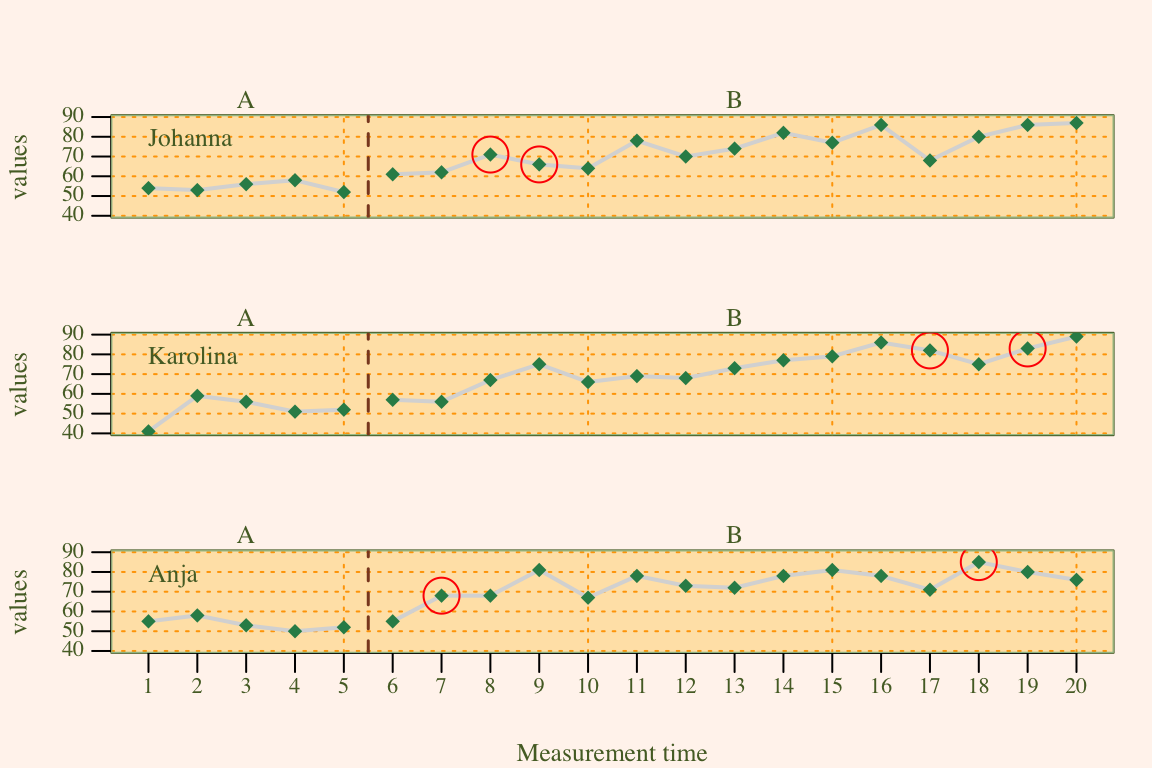
\includegraphics{scan-book_files/figure-latex/marks_example-1}

\}

\caption{Example of a plot with highlighted data-points}

(\#fig:marks\_example)
\textbackslash end\{figure\}

\hypertarget{graphical-styles-of-a-plot}{%
\section{Graphical styles of a plot}\label{graphical-styles-of-a-plot}}

The \texttt{style} argument of the plot function allows to specify a specific design of a plot. By default, the \texttt{grid} style is applied. \texttt{scan} includes some further predefined styles. \texttt{default,\ yaxis,\ tiny,\ small,\ big,\ chart,\ ridge,\ annotate,\ grid,\ grid2,\ dark,\ nodot,\ and\ sienna}. The name of a style is provided as a character string (e.g., \texttt{style\ =\ "grid"}).\\
Some styles only address specific elements (e.g., ``small'' or ``tiny'' just influence text and line sizes). These styles lend themselves to be combined with other style. This could be achieved by providing several style names to the plot argument: \texttt{style\ =\ c("grid",\ "annotate",\ "small")}.\\
Beyond predefined styles, styles can be individually modified and created. New styles are provided as a \texttt{list} of several design parameters that are passed to the \texttt{style} argument of the \texttt{plot} function. Table \ref{tab:table-style} shows all design parameter that could be defined.\\
To define a new style, first create a list containing a plain design. The \texttt{style\_plot} function returns such a list with the default values for a plain design (e.g., \texttt{mystyle\ \textless{}-\ style\_plot()}). Single design parameters can now be set by assigning a specific value within the list. For example, \texttt{newstyle\$fill\ \textless{}-\ "grey90"} will set the \texttt{fill} parameter to \texttt{"grey90"}. Alternatively, changes to the plain design can already by defined within the \texttt{style\_plot} function. To set a light-blue background color and also an orange grid, create the style \texttt{style\_plot(fill.bg\ =\ "lightblue",\ grid\ =\ "orange")}.
If you do not want to start with the plain design but a different of the predefined styles, set the \texttt{style} argument. If, for example, you like to have the \texttt{grid} combined with the \texttt{big} style but want to change the color of the grid to orange type \texttt{style\_plot(style\ =\ c("grid",\ "big"),\ col.grid\ =\ "orange")}. \texttt{plot(mydata,\ style\ =\ mystyle)} will apply the new style in a plot. Please note that the new style is not passed in quotation marks.

\begin{table}

\caption{\label{tab:table-style}Arguments of the style plot function}
\centering
\begin{tabular}[t]{>{\raggedright\arraybackslash}p{15em}>{\raggedright\arraybackslash}p{30em}}
\toprule
Argument & What it does ...\\
\midrule
\textbf{fill} & If TRUE area under the line is filled.\\
\textbf{col.fill} & Sets the color of the area under the line.\\
\textbf{grid} & If TRUE a grid is included.\\
\textbf{col.grid} & Sets the color of the grid.\\
\textbf{lty.grid} & Sets the line type of the grid.\\
\addlinespace
\textbf{lwd.grid} & Sets the line thikness of the grid.\\
\textbf{fill.bg} & If not NA the backgorund of the plot is filled with the given color.\\
\textbf{annotations} & A list of parameters defining annotations to each data point. This adds the score of each MT to your plot. `'pos'` Position of the annotations: 1 = below, 2 = left, 3 = above, 4 = right. `'col'` Color of the annotations. `'cex'` Size of the annotations. `'round'` rounds the values to the specified decimal. `annotations = list(pos = 3, col = 'brown', round = 1)` adds scores rounded to one decimal above the data point in brown color to the plot.\\
\textbf{text.ABlag} & By default a vertical line separates phases A and B in the plot. Alternatively, you could print a character string between the two phases using this argument: `text.ABlag = 'Start'`.\\
\textbf{lwd} & Width of the plot line. Default is `lwd = 2`.\\
\addlinespace
\textbf{pch} & Point type. Default is `pch = 17` (triangles). Other options are for example: 16 (filled circles) or 'A' (uses the letter A).\\
\textbf{col.lines} & The color of the lines. If set to an empty string no lines are drawn.\\
\textbf{col.dots} & The color of the dots. If set to an empty string no dots are drawn.\\
\textbf{mai} & Sets the margins of the plot.\\
\textbf{...} & Further arguments passed to the plot command.\\
\bottomrule
\end{tabular}
\end{table}

The width of the lines are set with the \texttt{lwd} argument, \texttt{col} is used to set the line colour and \texttt{pch} sets the symbol for a data point.
The \texttt{pch} argument can take several values for defining the symbol in which data points are plotted.

\begin{figure}
\centering
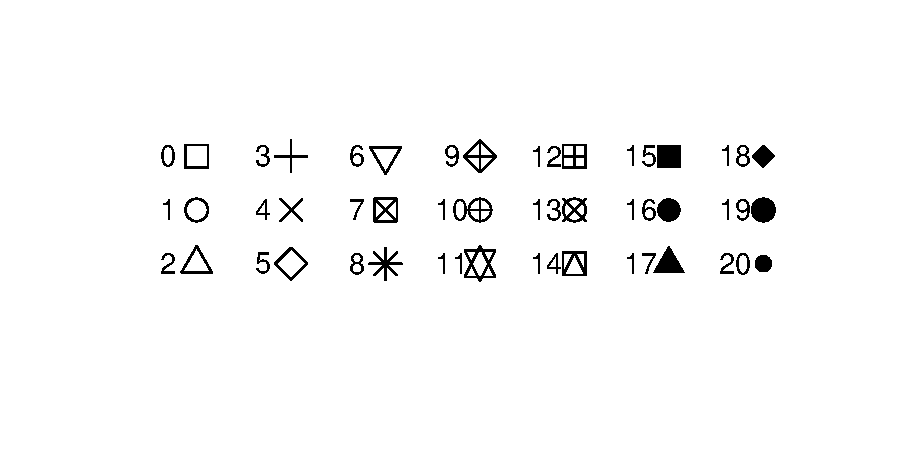
\includegraphics{scan-book_files/figure-latex/symbols, pch-1.pdf}
\caption{(\#fig:symbols, pch)Some of the possible symbols and their pch values.}
\end{figure}

Here is an example customizing a plot with several additional graphic parameters

\begin{Shaded}
\begin{Highlighting}[]
\NormalTok{newstyle }\OtherTok{\textless{}{-}} \FunctionTok{style\_plot}\NormalTok{(}\AttributeTok{fill =} \StringTok{"grey95"}\NormalTok{, }\AttributeTok{grid =} \StringTok{"lightblue"}\NormalTok{, }\AttributeTok{pch =} \DecValTok{16}\NormalTok{)}

\FunctionTok{plot}\NormalTok{(exampleABAB, }\AttributeTok{style =}\NormalTok{ newstyle)}
\end{Highlighting}
\end{Shaded}

\begin{figure}
\centering
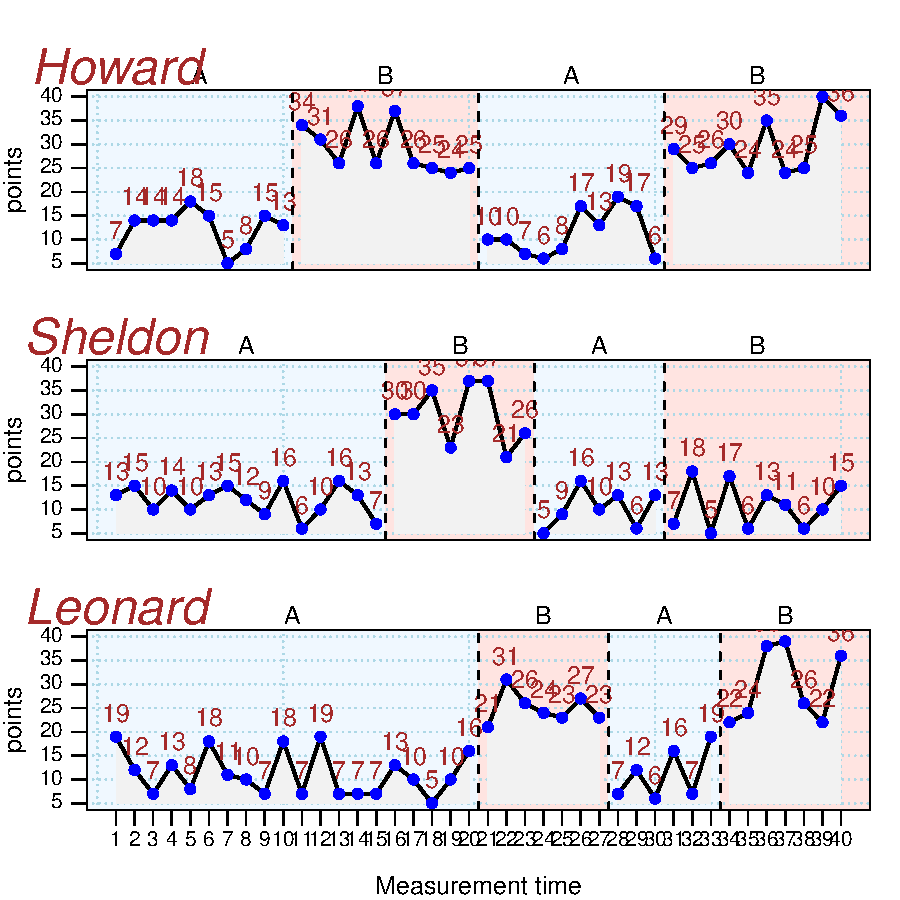
\includegraphics{scan-book_files/figure-latex/custom_style_example-1.pdf}
\caption{(\#fig:custom\_style\_example)A plot with a customized style.}
\end{figure}

\hypertarget{describe-and-manipulate-single-case-data-frames}{%
\chapter{Describe and manipulate single-case data frames}\label{describe-and-manipulate-single-case-data-frames}}

\hypertarget{describing-and-summarizing}{%
\section{Describing and summarizing}\label{describing-and-summarizing}}

A short description of the \emph{scdf} is provided by the \texttt{summary} command. The results are pretty much self explaining

\begin{Shaded}
\begin{Highlighting}[]
\FunctionTok{summary}\NormalTok{(Huber2014)}
\end{Highlighting}
\end{Shaded}

\begin{verbatim}
#A single-case data frame with 4 cases

          Measurements Design
Adam                37    A B
Berta               29    A B
Christian           76    A B
David               76    A B

Variable names:
mt <measurement-time variable>
compliance <dependent variable>
phase <phase variable>


Note:  Behavioral data (compliance in percent).
Author of data:  Christian Huber 
\end{verbatim}

\texttt{describe} is the basic command to get an overview on descriptive statistics. As an argument it only takes the name of the \emph{scdf} object. For each case of the \emph{scdf} and each phase within a case descriptive statistics are provided. The output table contains statistical indicators followed by a dot and the name of the phase (e.g., \texttt{n.A} for the number of measurements of phase A).

\begin{table}

\caption{\label{tab:table-describe}Statistics of the describeSC command}
\centering
\begin{tabular}[t]{>{\raggedright\arraybackslash}p{15em}>{\raggedright\arraybackslash}p{30em}}
\toprule
Parameter & What it means ...\\
\midrule
\textbf{n} & Number of measurements.\\
\textbf{mis} & Number of missing values.\\
\textbf{m} & Mean values.\\
\textbf{md} & Median of values.\\
\textbf{sd} & Standard deviation of values.\\
\addlinespace
\textbf{mad} & Median average deviation of values.\\
\textbf{min/max} & Min and max of values.\\
\textbf{trend} & Slope of a regression line through values by time.\\
\bottomrule
\end{tabular}
\end{table}

\begin{Shaded}
\begin{Highlighting}[]
\FunctionTok{describe}\NormalTok{(exampleABC)}
\end{Highlighting}
\end{Shaded}

\begin{verbatim}
Describe Single-Case Data

Design:  A B C 

        Marie Rosalind Lise
    n.A    10       15   20
    n.B    10        8    7
    n.C    10        7    3
  mis.A     0        0    0
  mis.B     0        0    0
  mis.C     0        0    0

        Marie Rosalind   Lise
    m.A 52.00    52.27  52.35
    m.B 72.10    73.25  73.57
    m.C 68.00    66.43  71.33
   md.A 53.50    52.00  52.00
   md.B 72.50    72.00  73.00
   md.C 69.00    68.00  76.00
   sd.A  8.29     8.15  10.87
   sd.B 11.37    13.13  10.64
   sd.C 12.70    10.49  21.39
  mad.A 11.12     7.41  10.38
  mad.B 10.38    10.38  16.31
  mad.C 17.79    11.86  20.76
  min.A 39.00    37.00  35.00
  min.B 47.00    54.00  60.00
  min.C 51.00    52.00  48.00
  max.A 63.00    65.00  74.00
  max.B 85.00    97.00  87.00
  max.C 87.00    78.00  90.00
trend.A -1.92     0.50  -0.09
trend.B -0.61     0.64   1.93
trend.C -0.19    -2.93 -14.00
\end{verbatim}

The resulting table could be exported into a csv file to be used in other software (e.g., to inserted in a word processing document). Therefore, first write the results of the \texttt{describeSC} command into an R object and then use the \texttt{write.csv} (or \texttt{write.csv2} for a German OS system setup) to export the \texttt{descriptives} element of the object.

\begin{Shaded}
\begin{Highlighting}[]
\CommentTok{\# write the results into a new R object named \textasciigrave{}res\textasciigrave{}}
\NormalTok{res }\OtherTok{\textless{}{-}} \FunctionTok{describe}\NormalTok{(exampleABC)}
\CommentTok{\# create a new file containing the descriptives on your harddrive}
\FunctionTok{write.csv}\NormalTok{(res}\SpecialCharTok{$}\NormalTok{descriptives, }\AttributeTok{file =} \StringTok{"descriptive data.csv"}\NormalTok{)}
\end{Highlighting}
\end{Shaded}

The file is written to the currently active working directory. If you are not sure where that is, type \texttt{getwd()} (you can use the \texttt{setwd()} command to define a different working directory. To get further details type \texttt{help(setwd)} into R).

\begin{rmdnote}
\textbf{Conflicting function names}\\
Sometimes R packages include the same function names. For example, the
\texttt{describe()} function is also part of the \texttt{psych} package.
Now, if you have loaded the \texttt{psych} package with
\texttt{library(psych)} after \texttt{scan} the \texttt{describe()}
function of scan will be masked (\texttt{describe()} would now call the
corresponding function of the \texttt{psych} package).\\
There are two solutions to this problem:

\begin{enumerate}
\def\labelenumi{\arabic{enumi}.}
\tightlist
\item
  activate the \texttt{psych} library before the \texttt{scan} library
  (now the psych \texttt{describe()} function will be masked) or
\item
  include the package name into the function call with the prefix
  \texttt{scan::}: \texttt{scan::describe()}.
\end{enumerate}
\end{rmdnote}

\hypertarget{autoregression-and-trendanalyses}{%
\section{Autoregression and trendanalyses}\label{autoregression-and-trendanalyses}}

The \texttt{autocorr} function calculates autocorrelations within each phase and across all phases. The \texttt{lag.max} argument defines the lag up to which the autocorrelation will be computed.

\begin{Shaded}
\begin{Highlighting}[]
\FunctionTok{autocorr}\NormalTok{(exampleABC, }\AttributeTok{lag.max =} \DecValTok{4}\NormalTok{)}
\end{Highlighting}
\end{Shaded}

\begin{verbatim}
Autocorrelations

     case phase lag_1 lag_2 lag_3 lag_4
    Marie     A  0.29 -0.11  0.10  0.12
    Marie     B -0.28 -0.10 -0.14 -0.09
    Marie     C  0.00 -0.33 -0.14 -0.25
    Marie   all  0.21  0.10  0.25  0.12
 Rosalind     A  0.37 -0.29 -0.33 -0.34
 Rosalind     B -0.34  0.24 -0.40  0.04
 Rosalind     C -0.07 -0.32  0.27  0.02
 Rosalind   all  0.49  0.38  0.22  0.17
     Lise     A  0.04 -0.32 -0.05 -0.09
     Lise     B -0.63  0.50 -0.40  0.31
     Lise     C -0.38 -0.12    NA    NA
     Lise   all  0.33  0.36  0.23  0.27
\end{verbatim}

The \texttt{trendSC} function provides an overview of linear trends in single-case data. By default, it gives you the intercept and slope of a linear and a squared regression of measurement-time on scores. Models are computed separately for each phase and across all phases. For a more advanced application, you can add regression models using the R specific formula class.

\begin{Shaded}
\begin{Highlighting}[]
\CommentTok{\# Simple example}
\FunctionTok{trend}\NormalTok{(exampleABC[}\DecValTok{1}\NormalTok{])}
\end{Highlighting}
\end{Shaded}

\begin{verbatim}
Trend for each phase

            Intercept      B   Beta
Linear.ALL     55.159  0.612  0.392
Linear.A       60.618 -1.915 -0.700
Linear.B       74.855 -0.612 -0.163
Linear.C       68.873 -0.194 -0.046
Squared.ALL    59.135  0.017  0.330
Squared.A      57.937 -0.208 -0.712
Squared.B      73.217 -0.039 -0.098
Squared.C      68.490 -0.017 -0.038

Note. Measurement-times of phase B start at 0 
\end{verbatim}

\begin{Shaded}
\begin{Highlighting}[]
\CommentTok{\# Complex example}
\FunctionTok{trend}\NormalTok{(exampleAB}\SpecialCharTok{$}\NormalTok{Johanna, }\AttributeTok{offset =} \DecValTok{0}\NormalTok{, }
        \AttributeTok{model =} \FunctionTok{c}\NormalTok{(}\StringTok{"Cubic"} \OtherTok{=}\NormalTok{ values }\SpecialCharTok{\textasciitilde{}} \FunctionTok{I}\NormalTok{(mt}\SpecialCharTok{\^{}}\DecValTok{3}\NormalTok{), }\StringTok{"Log Time"} \OtherTok{=}\NormalTok{ values }\SpecialCharTok{\textasciitilde{}} \FunctionTok{log}\NormalTok{(mt))}
\NormalTok{)}
\end{Highlighting}
\end{Shaded}

\begin{verbatim}
Trend for each phase

             Intercept      B   Beta
Linear.ALL      50.484  1.787  0.908
Linear.A        54.300  0.100  0.066
Linear.B        61.133  1.625  0.813
Squared.ALL     57.879  0.079  0.871
Squared.A       54.747 -0.013 -0.054
Squared.B       66.343  0.094  0.775
Cubic.ALL       60.886  0.004  0.816
Cubic.A         54.959 -0.008 -0.169
Cubic.B         68.368  0.006  0.732
Log Time.ALL    43.532 12.149  0.848
Log Time.A      54.032  0.593  0.156
Log Time.B      57.300  9.051  0.791

Note. Measurement-times of phase B start at 1 
\end{verbatim}

\hypertarget{missing-values}{%
\section{Missing values}\label{missing-values}}

There are two kinds of missing values in single-case data series. First, missings that were explicitly recorded as \texttt{NA} and assigned to a phase and measurement-time as in the following example:

\begin{verbatim}
scdf(c(5, 3, 4, 6, 8, 7, 9, 7, NA, 6), phase.design = c(A = 4, B = 6))
\end{verbatim}

The second type of missing occurs when there are gaps between measurement-times that are not explicitly coded as in the following example:

\begin{verbatim}
scdf(c(5, 3, 4, 6, 8, 7, 9, 7, 6), phase.design = c(A = 4, B = 5), 
     mt = c(1, 2, 3, 4, 5, 6, 7, 8, 10))
\end{verbatim}

In both cases, missing values pose a threat to the internal validity of overlap indices. Randomization tests are more robust against the first type of missing values but are affected by the second type. Regression approaches are less impacted by both types as they take the interval between measurement-times into account.

\begin{Shaded}
\begin{Highlighting}[]
\NormalTok{case1 }\OtherTok{\textless{}{-}} \FunctionTok{scdf}\NormalTok{(}\FunctionTok{c}\NormalTok{(}\DecValTok{3}\NormalTok{,}\DecValTok{6}\NormalTok{,}\DecValTok{2}\NormalTok{,}\DecValTok{4}\NormalTok{,}\DecValTok{3}\NormalTok{,}\DecValTok{5}\NormalTok{,}\DecValTok{2}\NormalTok{,}\DecValTok{6}\NormalTok{,}\DecValTok{3}\NormalTok{,}\DecValTok{2}\NormalTok{, }\DecValTok{6}\NormalTok{,}\DecValTok{7}\NormalTok{,}\DecValTok{5}\NormalTok{,}\DecValTok{8}\NormalTok{,}\DecValTok{6}\NormalTok{,}\DecValTok{7}\NormalTok{,}\DecValTok{4}\NormalTok{,}\DecValTok{8}\NormalTok{,}\DecValTok{5}\NormalTok{,}\DecValTok{6}\NormalTok{), }
              \AttributeTok{phase.design =} \FunctionTok{c}\NormalTok{(}\AttributeTok{A =} \DecValTok{10}\NormalTok{, }\AttributeTok{B =} \DecValTok{10}\NormalTok{), }\AttributeTok{name =} \StringTok{"no NA"}\NormalTok{)}
\NormalTok{case2 }\OtherTok{\textless{}{-}} \FunctionTok{scdf}\NormalTok{(}\FunctionTok{c}\NormalTok{(}\DecValTok{3}\NormalTok{,}\DecValTok{6}\NormalTok{,}\DecValTok{2}\NormalTok{,}\DecValTok{4}\NormalTok{,}\DecValTok{3}\NormalTok{,}\DecValTok{5}\NormalTok{,}\DecValTok{2}\NormalTok{,}\ConstantTok{NA}\NormalTok{,}\DecValTok{3}\NormalTok{,}\DecValTok{2}\NormalTok{, }\DecValTok{6}\NormalTok{,}\DecValTok{7}\NormalTok{,}\DecValTok{5}\NormalTok{,}\DecValTok{8}\NormalTok{,}\DecValTok{6}\NormalTok{,}\ConstantTok{NA}\NormalTok{,}\DecValTok{4}\NormalTok{,}\DecValTok{8}\NormalTok{,}\DecValTok{5}\NormalTok{,}\DecValTok{6}\NormalTok{), }
              \AttributeTok{phase.design =} \FunctionTok{c}\NormalTok{(}\AttributeTok{A =} \DecValTok{10}\NormalTok{, }\AttributeTok{B =} \DecValTok{10}\NormalTok{), }\AttributeTok{name =} \StringTok{"NAs"}\NormalTok{)}
\NormalTok{case3 }\OtherTok{\textless{}{-}} \FunctionTok{fillmissingSC}\NormalTok{(case2)}
\FunctionTok{names}\NormalTok{(case3) }\OtherTok{\textless{}{-}} \StringTok{"interpolated NAs"}
\NormalTok{ex }\OtherTok{\textless{}{-}} \FunctionTok{c}\NormalTok{(case1, case2, case3)}
\FunctionTok{plot}\NormalTok{(ex)}
\end{Highlighting}
\end{Shaded}

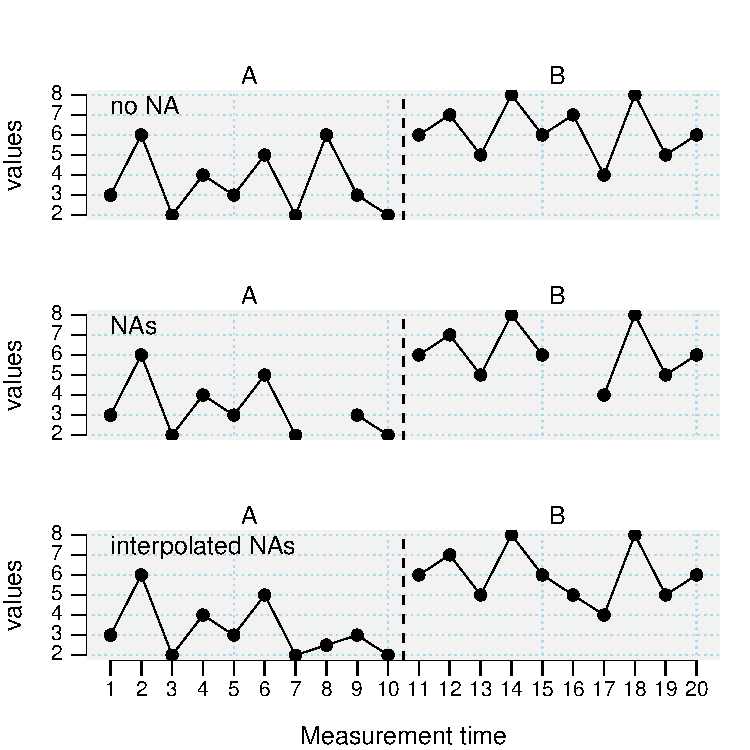
\includegraphics{scan-book_files/figure-latex/fillmissing_example-1.pdf}

\begin{Shaded}
\begin{Highlighting}[]
\FunctionTok{overlap}\NormalTok{(ex)}
\end{Highlighting}
\end{Shaded}

\begin{verbatim}
Overlap Indices

Design:  A B 
Comparing phase 1 against phase 2 

              no NA    NAs interpolated NAs
PND           40.00  33.33            30.00
PEM          100.00 100.00           100.00
PET          100.00 100.00           100.00
NAP           88.50  91.36            91.50
NAP.rescaled  77.00  82.72            83.00
PAND          72.50  80.56            80.00
TAU_U          0.45   0.51             0.50
Base_Tau       0.59   0.64             0.64
Diff_mean      2.60   2.78             2.75
Diff_trend     0.02   0.11             0.12
SMD            1.65   1.96             2.02
\end{verbatim}

\hypertarget{outlieranalysis}{%
\section{Outlieranalysis}\label{outlieranalysis}}

\emph{scan} provides several methods for analyzing outliers. All of them are implemented in the \texttt{outliers} function. Available methods are the \textbf{standard deviation}, \textbf{mean average deviation}, \textbf{confidence intervals}, and \textbf{Cook's distance}. The criteria argument takes a vector with two information, the first defines the analyzing method (``SD,'' ``MAD,'' CI``,''Cook``) and the second the criteria. For''SD" the criteria is the number of standard deviations (\textbf{sd}) from the mean of each phase for which a value is not considered to be an outlier. For example, \texttt{criteria\ =\ c("SD",2)} would identify every value exceeding two \textbf{sd} above or below the mean as an outlier whereas \textbf{sd} and mean refer to phase of a value. As this might be misleading particularly for small samples Iglewicz and Hoaglin \protect\hyperlink{ref-iglewicz_how_1993}{Iglewicz \& Hoaglin} (\protect\hyperlink{ref-iglewicz_how_1993}{1993}) recommend the use the much more robust median average deviation (\textbf{MAD}) instead. The \textbf{MAD} is is constructed similar to the \textbf{sd} but uses the median instead of the mean. Multiplying the \textbf{MAD} by 1.4826 approximates the \textbf{sd} in a normal distributed sample. This corrected MAD is applied in the \texttt{outlier} function. A deviation of 3.5 times the corrected \textbf{MAD} from the median is suggested to be an outlier. To use this criterion set \texttt{criteria\ =\ c("MAD",\ 3.5)}. \texttt{criteria\ =\ c("CI",\ 0.95)} takes exceeding the 95\% confidence interval as the criteria for outliers. The Cook's distance method for calculation outliers can be applied with a strict AB-phase design. in that case, the Cook's distance analyses are based on a piecewise-regression model. Most commonly, Cook's distance exceeding 4/n is used as a criteria. This could be implemented setting `criteria = c(``Cook,''``4/n'').

\begin{Shaded}
\begin{Highlighting}[]
\FunctionTok{outlier}\NormalTok{(exampleABC\_outlier, }\AttributeTok{criteria =} \FunctionTok{c}\NormalTok{(}\StringTok{"MAD"}\NormalTok{, }\FloatTok{3.5}\NormalTok{))}
\end{Highlighting}
\end{Shaded}

\begin{verbatim}
Outlier Analysis for Single-Case Data

Criteria: Exceeds 3.5 Mean Average Deviations

$Bernadette
  phase md mad   lower    upper
1     A 57   9 10.2981 103.7019
2     B 76   7 39.6763 112.3237
3     C 69  12  6.7308 131.2692

$Penny
  phase md mad   lower    upper
1     A 52   6 20.8654  83.1346
2     B 74  10 22.1090 125.8910
3     C 68   8 26.4872 109.5128

$Amy
  phase md mad   lower    upper
1     A 54   9  7.2981 100.7019
2     B 73  11 15.9199 130.0801
3     C 76  14  3.3526 148.6474

Case Bernadette : Dropped 3 
Case Penny : Dropped 2 
Case Amy : Dropped 3 
\end{verbatim}

\begin{Shaded}
\begin{Highlighting}[]
\CommentTok{\# Visualizing outliers with the plot function}
\NormalTok{res }\OtherTok{\textless{}{-}} \FunctionTok{outlier}\NormalTok{(exampleABC\_outlier, }\AttributeTok{criteria =} \FunctionTok{c}\NormalTok{(}\StringTok{"MAD"}\NormalTok{, }\FloatTok{3.5}\NormalTok{))}
\FunctionTok{plot}\NormalTok{(exampleABC\_outlier, }\AttributeTok{marks =}\NormalTok{ res, }\AttributeTok{style =} \StringTok{"annotate"}\NormalTok{, }\AttributeTok{ylim =} \FunctionTok{c}\NormalTok{(}\DecValTok{40}\NormalTok{,}\DecValTok{160}\NormalTok{))}
\end{Highlighting}
\end{Shaded}

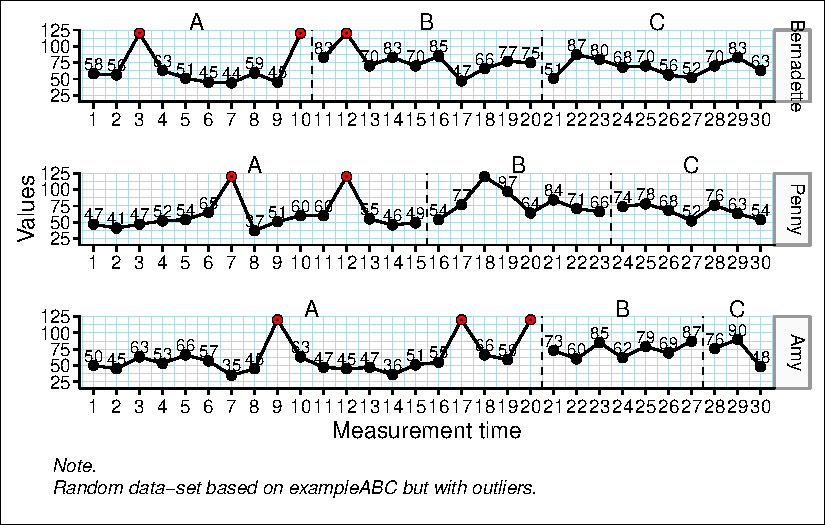
\includegraphics{scan-book_files/figure-latex/outlier-1.pdf}

\hypertarget{smoothing-data}{%
\section{Smoothing data}\label{smoothing-data}}

The \texttt{smooth\_cases} function provides procedures to smooth single-case data and eliminate noise. A moving average function (mean- or median-based) replaces each data point by the average of the surrounding data points step-by-step. A \emph{lag} defines the number of measurements before and after the calculation is based on. So a lag-1 will take the average of the proceeding and following value and lag-2 the average of the two proceeding and two following measurements. With a local regression function, each data point is regressed by its surrounding data points. Here, the proportion of measurements surrounding a value is usually defined. So an intensity of 0.2 will take the surrounding 20\% of data as the basis for a regression.\\
The function returns am scdf with smoothed data points.

\begin{Shaded}
\begin{Highlighting}[]
\DocumentationTok{\#\# Use the three different smoothing functions and compare the results}
\NormalTok{berta\_mmd }\OtherTok{\textless{}{-}} \FunctionTok{smooth\_cases}\NormalTok{(Huber2014}\SpecialCharTok{$}\NormalTok{Berta)}
\NormalTok{berta\_mmn }\OtherTok{\textless{}{-}} \FunctionTok{smooth\_cases}\NormalTok{(Huber2014}\SpecialCharTok{$}\NormalTok{Berta, }\AttributeTok{FUN =} \StringTok{"movingMean"}\NormalTok{)}
\NormalTok{berta\_lre }\OtherTok{\textless{}{-}} \FunctionTok{smooth\_cases}\NormalTok{(Huber2014}\SpecialCharTok{$}\NormalTok{Berta, }\AttributeTok{FUN =} \StringTok{"localRegression"}\NormalTok{)}
\NormalTok{new\_study }\OtherTok{\textless{}{-}} \FunctionTok{c}\NormalTok{(Huber2014}\SpecialCharTok{$}\NormalTok{Berta, berta\_mmd, berta\_mmn, berta\_lre)}
\FunctionTok{names}\NormalTok{(new\_study) }\OtherTok{\textless{}{-}} \FunctionTok{c}\NormalTok{(}\StringTok{"Original"}\NormalTok{, }\StringTok{"Moving Median"}\NormalTok{, }\StringTok{"Moving Mean"}\NormalTok{, }\StringTok{"Local Regression"}\NormalTok{)}
\FunctionTok{plot}\NormalTok{(new\_study, }\AttributeTok{style =} \StringTok{"grid2"}\NormalTok{)}
\end{Highlighting}
\end{Shaded}

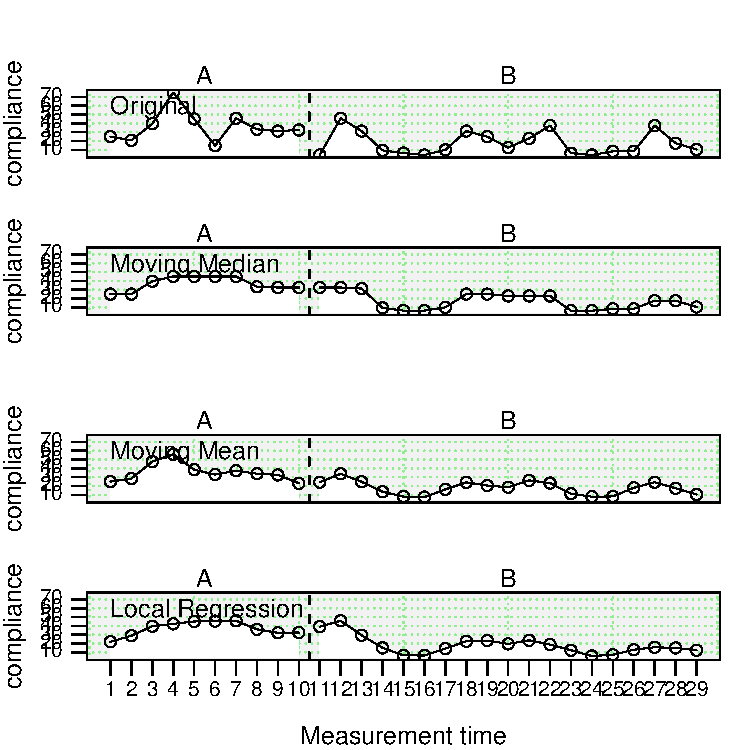
\includegraphics{scan-book_files/figure-latex/smooth_example-1.pdf}

\hypertarget{overlapping-indices}{%
\chapter{Overlapping indices}\label{overlapping-indices}}

\texttt{overlap} provides a table with some of the most important overlap indices for each case of an \emph{scdf}. For calculating overlap indicators is is important to know if a decrease or an increase of values is expected between phases. By default \texttt{overlap} assumes an increase in values. If the argument \texttt{decreasing\ =\ TRUE} is set, calculation will be based on the assumption of decreasing values.

\begin{Shaded}
\begin{Highlighting}[]
\FunctionTok{overlap}\NormalTok{(exampleAB)}
\end{Highlighting}
\end{Shaded}

\begin{verbatim}
Overlap Indices

Design:  A B 
Comparing phase 1 against phase 2 

             Johanna Karolina   Anja
PND           100.00    86.67  93.33
PEM           100.00   100.00 100.00
PET           100.00    93.33 100.00
NAP           100.00    96.67  98.00
NAP.rescaled  100.00    93.33  96.00
PAND          100.00    90.00  90.00
TAU_U           0.77     0.78   0.64
Base_Tau        0.63     0.59   0.61
Diff_mean      19.53    21.67  20.47
Diff_trend      1.53     0.54   2.50
SMD             8.11     3.17   6.71
\end{verbatim}

Overlap measures refer to a comparison of two phases within a single-case data-set. By default, \texttt{overlap} compares a Phase A to a Phase B. The \texttt{phases} argument is needed if the phases of the \emph{scdf} do not include phases named A and B or a comparison between other phases in wanted.\\
The \texttt{phases} argument takes a list with two elements. One element for each of the two phases that should be compared. The elements could contain either the name of the two phases or the number of the position within the \emph{scdf}. If you want to compare the first to the third phase you can set \texttt{phases\ =\ list(1,3)}. If the phases of your case are named `A,' `B,' and `C' you could alternatively set \texttt{phases\ =\ list("A","C")}.\\
It is also possible to compare a combination of several cases against a combination of other phases. Each of the two list-elements could contain more than one phase which are concatenated with the \texttt{c} command. For example if you have an ABAB-Design and like to compare the two A-phases against the two B-phases \texttt{phases\ =\ list(\ c(1,3),\ c(2,4)\ )} will do the trick.

\begin{Shaded}
\begin{Highlighting}[]
\FunctionTok{overlap}\NormalTok{(exampleA1B1A2B2, }\AttributeTok{phases =} \FunctionTok{list}\NormalTok{( }\FunctionTok{c}\NormalTok{(}\StringTok{"A1"}\NormalTok{,}\StringTok{"A2"}\NormalTok{), }\FunctionTok{c}\NormalTok{(}\StringTok{"B1"}\NormalTok{,}\StringTok{"B2"}\NormalTok{)))}
\end{Highlighting}
\end{Shaded}

\begin{verbatim}
Overlap Indices

Design:  A1 B1 A2 B2 
Comparing phases 1 + 3 against phases 2 + 4 

              Pawel Moritz Jannis
PND           55.00  77.78  71.43
PEM          100.00 100.00 100.00
PET          100.00 100.00 100.00
NAP           94.50  96.84  98.35
NAP.rescaled  89.00  93.69  96.70
PAND          82.50  85.00  90.00
TAU_U          0.45   0.46   0.38
Base_Tau       0.65   0.68   0.68
Diff_mean     12.25  13.58  15.27
Diff_trend    -0.05   0.00  -0.54
SMD            2.68   3.27   3.62
\end{verbatim}

\hypertarget{percentage-non-overlapping-data-pnd}{%
\section{Percentage non-overlapping data (PND)}\label{percentage-non-overlapping-data-pnd}}

The percentage of non-overlapping data (PND) effect size measure was described by \protect\hyperlink{ref-scruggs_quantitative_1987}{Scruggs, Mastropieri, \& Casto} (\protect\hyperlink{ref-scruggs_quantitative_1987}{1987}) . It is the percentage of all data-points of the second phase of a single-case study exceeding the maximum value of the first phase. In case you have a study where you expect a decrease of values in the second phase, PND is calculated as the percentage of data-point of the second phase below the minimum of the first phase.

\begin{figure}
\centering
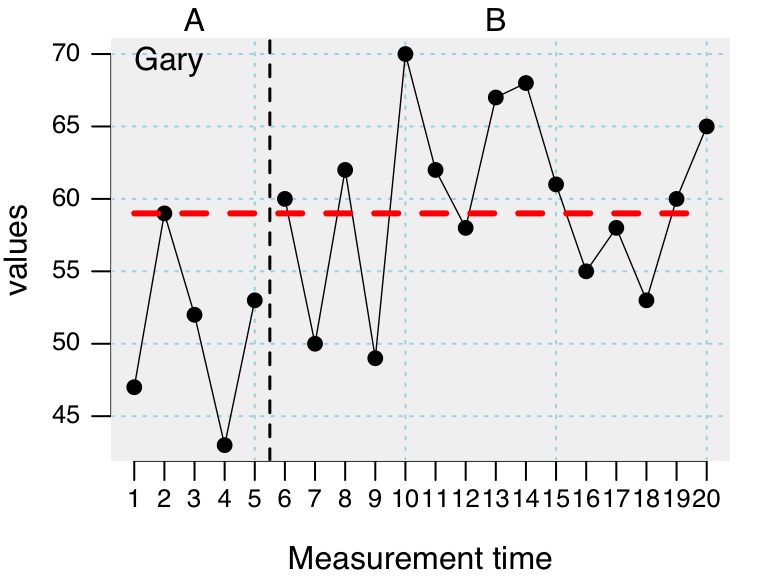
\includegraphics{scan-book_files/figure-latex/unnamed-chunk-25-1.pdf}
\caption{\label{fig:unnamed-chunk-25}Illustration of PND. PND is 60\% as 9 out of 15 datapoints of phase B are higher than the maximum of phase A.}
\end{figure}

The function \texttt{pnd} provides the PND for each case as well as the mean of all PNDs of that \emph{scdf}. When you expect decreasing values set \texttt{decreasing\ =\ TRUE}. When there are more than two phases or phases are not named A and B, use the \texttt{phases} argument as described at the beginning of this chapter.

\begin{Shaded}
\begin{Highlighting}[]
\FunctionTok{pnd}\NormalTok{(exampleAB)}
\end{Highlighting}
\end{Shaded}

\begin{verbatim}
Percent Non-Overlapping Data

     Case    PND Total Exceeds
  Johanna   100%    15      15
 Karolina 86.67%    15      13
     Anja 93.33%    15      14

Mean  : 93.33 %
\end{verbatim}

\hypertarget{percentage-exceeding-the-median-pem}{%
\section{Percentage exceeding the median (PEM)}\label{percentage-exceeding-the-median-pem}}

The pem function returns the percentage of phase B data exceeding the phase A median. Additionally, a binomial test against a 50/50 distribution is computed. Different measures of central tendency can be addressed for alternative analyses.

\begin{figure}
\centering
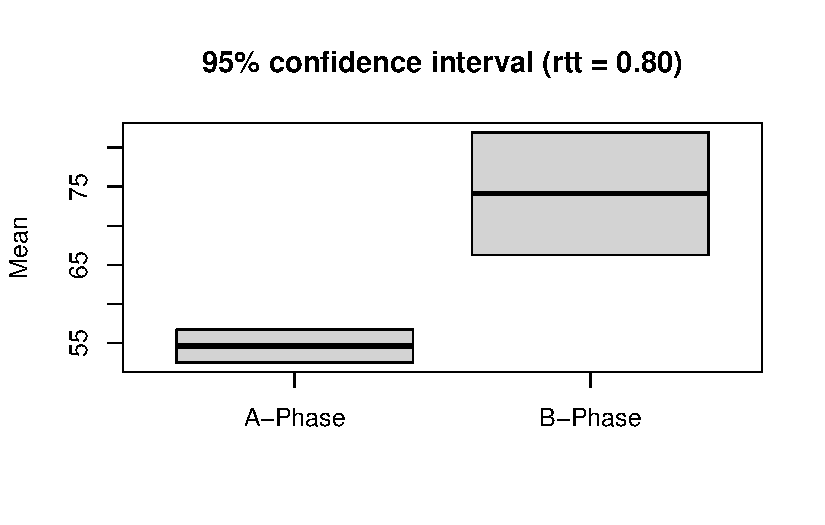
\includegraphics{scan-book_files/figure-latex/unnamed-chunk-28-1.pdf}
\caption{\label{fig:unnamed-chunk-28}Illustration of PEM. PEM is 75\% as 9 out of 12 datapoints of phase B are higher than the median of phase A.}
\end{figure}

\begin{Shaded}
\begin{Highlighting}[]
\FunctionTok{pem}\NormalTok{(exampleAB)}
\end{Highlighting}
\end{Shaded}

\begin{verbatim}
Percent Exceeding the Median

         PEM positives total binom.p
Johanna  100        15    15       0
Karolina 100        15    15       0
Anja     100        15    15       0

Alternative hypothesis: true probability > 50%
\end{verbatim}

\hypertarget{percentage-exceeding-the-regression-trend-pet}{%
\section{Percentage exceeding the regression trend (PET)}\label{percentage-exceeding-the-regression-trend-pet}}

The pet function provides the percentage of phase B data points exceeding the prediction based on the phase A trend. A binomial test against a 50/50 distribution is computed. Furthermore, the percentage of phase B data points exceeding the upper (or lower) 95 percent confidence interval of the predicted progress is computed.

\begin{Shaded}
\begin{Highlighting}[]
\FunctionTok{pet}\NormalTok{(exampleAB)}
\end{Highlighting}
\end{Shaded}

\begin{verbatim}
Percent Exceeding the Trend

N cases =  3 

             PET binom.p  PET CI
Johanna  100.000       0  86.667
Karolina  93.333       0   0.000
Anja     100.000       0 100.000

Binom.test: alternative hypothesis: true probability > 50%
PET CI: Percent of values greater than upper 95% confidence threshold (greater 1.645*se above predicted value)
\end{verbatim}

\begin{figure}
\centering
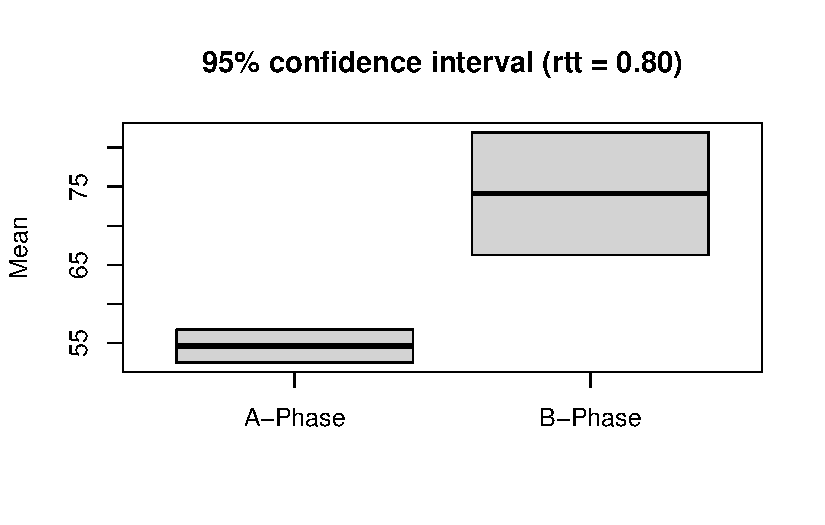
\includegraphics{scan-book_files/figure-latex/unnamed-chunk-32-1.pdf}
\caption{\label{fig:unnamed-chunk-32}Illustration of PET. PET is 66.7\% as 10 out of 15 datapoints of phase B are higher than the projected trend-line of phase A.}
\end{figure}

\hypertarget{percentage-of-all-non-overlapping-data-pand}{%
\section{Percentage of all non-overlapping data (PAND)}\label{percentage-of-all-non-overlapping-data-pand}}

The \texttt{pand} function calculates the percentage of all non-overlapping data (\protect\hyperlink{ref-parker_percentage_2007}{Richard I. Parker, Hagan-Burke, \& Vannest, 2007}), an index to quantify a level increase (or decrease) in performance after the onset of an intervention. The argument \texttt{correction\ =\ TRUE} makes \texttt{pand} use a frequency matrix, which is corrected for ties. A tie is counted as the half of a measurement in both phases. Set \texttt{correction\ =\ FALSE} to use the uncorrected matrix, which is not recommended.

\begin{Shaded}
\begin{Highlighting}[]
\FunctionTok{pand}\NormalTok{(exampleAB)}
\end{Highlighting}
\end{Shaded}

\begin{verbatim}
Percentage of all non-overlapping data

PAND =  93.3 %
F =  0.822  ; F² =  0.676 

Number of Cases: 3 
Total measurements: 60  (in phase A: 15; in phase B: 45)
n overlapping data per case: 0, 2, 2
Total overlapping data: n = 4 ; percentage = 6.7 

2 x 2 Matrix of proportions
    % expected
    A   B   total
%    A  21.7    3.3 25
real B  3.3 71.7    75
 total  25  75

2 x 2 Matrix of counts
    expected
    A   B   total
     A  13  2   15
real B  2   43  45
 total  15  45


Note. Matrix is corrected for ties

Correlation based analysis:

z = 6.316, p = 0.000, t = 0.822 
\end{verbatim}

PAND indicates nonoverlap between phase A and B data (like PND), but uses all data and is therefore not based on one single (probably unrepresentative) datapoint. Furthermore, PAND allows the comparison of real and expected associations (Chi-square test) and estimation of the effect size Phi, which equals Pearsons r for dichotomous data. Thus, phi-Square is the amount of explained variance. The original procedure for computing PAND does not account for ambivalent datapoints (ties). The newer NAP overcomes this problem and has better precision-power (\protect\hyperlink{ref-parker_effect_2011}{Richard I. Parker, Vannest, \& Davis, 2011}).

\hypertarget{nonoverlap-of-all-pairs-nap}{%
\section{Nonoverlap of all pairs (NAP)}\label{nonoverlap-of-all-pairs-nap}}

The \texttt{nap} function calculates the nonoverlap of all pairs (\protect\hyperlink{ref-parker_improved_2009}{Richard I. Parker \& Vannest, 2009}). NAP summarizes the overlap between all pairs of phase A and phase B data points. If an increase of phase B scores is expected, a non-overlapping pair has a higher phase B data point. The NAP equals number of pairs showing no overlap / number of pairs. Because NAP can only take values between 50 and 100 percent, a rescaled and therefore more intuitive NAP (0-100\%) is also displayed. NAP is equivalent to the the U-test and Wilcox rank sum test. Thus, a Wilcox test is conducted and reported for each case.

\begin{Shaded}
\begin{Highlighting}[]
\FunctionTok{nap}\NormalTok{(exampleAB)}
\end{Highlighting}
\end{Shaded}

\begin{verbatim}
Nonoverlap of All Pairs

     Case NAP Rescaled Pairs Positives Ties   W       p
  Johanna 100      100    75        75    0 0.0 0.00062
 Karolina  97       93    75        72    1 2.5 0.00129
     Anja  98       96    75        73    1 1.5 0.00095
\end{verbatim}

\hypertarget{tau-u}{%
\section{Tau-U}\label{tau-u}}

The \texttt{tau\_u} function takes a \emph{scdf} and returns Tau-U calculations for each single-case within that file. Additionally, an overall Tau-U value is calculated for all cases. The overall Tau-U value is the average of all Tau-U values weighted by their standard error. This procedure has been proposed by \protect\hyperlink{ref-parker_combining_2011}{Richard I. Parker, Vannest, Davis, \& Sauber} (\protect\hyperlink{ref-parker_combining_2011}{2011}).\\
The \texttt{tau\_u} function provides two methods for calculation of Tau-U. By setting the argument \texttt{method\ =\ "parker"}, Tau-U is calculated as described in \protect\hyperlink{ref-parker_combining_2011}{Richard I. Parker, Vannest, Davis, \& Sauber} (\protect\hyperlink{ref-parker_combining_2011}{2011}). This procedure could lead to Tau-U values above 1 and below -1 which are difficult to interpret. \texttt{method\ =\ "complete}, which is the default, applies a correction that keeps the values within the -1 to 1 range and should be more appropriate.\\
In the method proposed by \protect\hyperlink{ref-parker_combining_2011}{Richard I. Parker, Vannest, Davis, \& Sauber} (\protect\hyperlink{ref-parker_combining_2011}{2011}) data of the same value (ties) are ignored and treated as if these data had not been available. Alternatively, ties might be considered in favor of the intervention or not. For the latter, the \texttt{ties.method} argument could be set to \texttt{ties.method\ =\ "positive"} or \texttt{ties.method\ =\ "negative"}. The default is \texttt{"omit"} following \protect\hyperlink{ref-parker_combining_2011}{Richard I. Parker, Vannest, Davis, \& Sauber} (\protect\hyperlink{ref-parker_combining_2011}{2011}).\\
The standard return of the \texttt{tau\_u} function does not display all calculations. If you like to have more details, apply the \texttt{print} function with the additional argument \texttt{complete\ =\ TRUE}.

\begin{Shaded}
\begin{Highlighting}[]
\NormalTok{dat }\OtherTok{\textless{}{-}} \FunctionTok{scdf}\NormalTok{(}\FunctionTok{c}\NormalTok{(}\DecValTok{2}\NormalTok{,}\DecValTok{0}\NormalTok{,}\DecValTok{1}\NormalTok{,}\DecValTok{4}\NormalTok{,}\DecValTok{3}\NormalTok{,}\DecValTok{5}\NormalTok{,}\DecValTok{9}\NormalTok{,}\DecValTok{7}\NormalTok{,}\DecValTok{8}\NormalTok{), }\AttributeTok{phase.design =} \FunctionTok{c}\NormalTok{(}\AttributeTok{A =} \DecValTok{4}\NormalTok{, }\AttributeTok{B =} \DecValTok{5}\NormalTok{))}
\NormalTok{res }\OtherTok{\textless{}{-}} \FunctionTok{tau\_u}\NormalTok{(dat)}
\FunctionTok{print}\NormalTok{(res, }\AttributeTok{complete =} \ConstantTok{TRUE}\NormalTok{)}
\end{Highlighting}
\end{Shaded}

\begin{verbatim}
Tau-U
Method:  complete 

Overall Tau-U: 
                       Model Tau_U     se     z df        p
                     A vs. B 0.900 0.0672 13.40  0 6.23e-41
           A vs. B - Trend A 0.523 0.2569  2.04  0 4.17e-02
           A vs. B + Trend B 0.730 0.1650  4.43  0 9.59e-06
 A vs. B + Trend B - Trend A 0.611 0.2215  2.76  0 5.80e-03

$Case1
                            kendall    k_p n pairs pos neg ties  S    D   Tau
A vs. B                       0.671 0.0373 9    20  19   1    0 18 20.0 0.900
Trend A                       0.333 0.7341 4     6   4   2    0  2  6.0 0.333
Trend B                       0.600 0.2207 5    10   8   2    0  6 10.0 0.600
A vs. B - Trend A             0.523 0.0839 9    26  21   5    0 16 30.6 0.523
A vs. B + Trend B             0.730 0.0118 9    30  27   3    0 24 32.9 0.730
A vs. B + Trend B - Trend A   0.611 0.0286 9    36  29   7    0 22 36.0 0.611
                            SD_S VAR_S SE_Tau     Z       p
A vs. B                     8.16 66.67  0.408 2.205 0.02749
Trend A                     2.94  8.67  0.491 0.679 0.49691
Trend B                     4.08 16.67  0.408 1.470 0.14164
A vs. B - Trend A           8.68 75.33  0.284 1.843 0.06527
A vs. B + Trend B           9.13 83.33  0.278 2.629 0.00856
A vs. B + Trend B - Trend A 9.59 92.00  0.266 2.294 0.02181
\end{verbatim}

\begin{Shaded}
\begin{Highlighting}[]
\FunctionTok{tau\_u}\NormalTok{(exampleAB)}
\end{Highlighting}
\end{Shaded}

\begin{verbatim}
Tau-U
Method:  complete 

Overall Tau-U: 
                       Model Tau_U     se    z df        p
                     A vs. B 0.960 0.0132 72.8  2 0.00e+00
           A vs. B - Trend A 0.593 0.0859  6.9  2 5.33e-12
           A vs. B + Trend B 0.770 0.0547 14.1  2 5.04e-45
 A vs. B + Trend B - Trend A 0.750 0.0585 12.8  2 1.21e-37

$Johanna
                              Tau SE_Tau    Z     p
A vs. B                     1.000  0.306 3.27 0.001
A vs. B - Trend A           0.592  0.184 3.22 0.001
A vs. B + Trend B           0.786  0.166 4.75 0.000
A vs. B + Trend B - Trend A 0.765  0.163 4.71 0.000

$Karolina
                              Tau SE_Tau    Z     p
A vs. B                     0.940  0.308 3.06 0.002
A vs. B - Trend A           0.554  0.184 3.01 0.003
A vs. B + Trend B           0.805  0.166 4.85 0.000
A vs. B + Trend B - Trend A 0.783  0.163 4.81 0.000

$Anja
                              Tau SE_Tau    Z     p
A vs. B                     0.966  0.308 3.14 0.002
A vs. B - Trend A           0.624  0.186 3.36 0.001
A vs. B + Trend B           0.626  0.167 3.74 0.000
A vs. B + Trend B - Trend A 0.642  0.164 3.91 0.000
\end{verbatim}

\hypertarget{reliable-change-index}{%
\section{Reliable change index}\label{reliable-change-index}}

Basically, the reliable change index (rci) depicts if a post-test is above a pre-test value. Based on the reliability of the measurements and the standard-deviation the standard error is calculated. The mean difference between phase-A and phase-B is divided by the standard-error. Several authors proposed refined methods for calculating the rci.

The \texttt{rci} function computes three indices of reliable change (\protect\hyperlink{ref-wise_methods_2004}{Wise, 2004}) and corresponding descriptive statistics.

\begin{Shaded}
\begin{Highlighting}[]
\FunctionTok{rci}\NormalTok{(exampleAB}\SpecialCharTok{$}\NormalTok{Johanna, }\AttributeTok{rel =} \FloatTok{0.8}\NormalTok{, }\AttributeTok{graph =} \ConstantTok{TRUE}\NormalTok{)}
\end{Highlighting}
\end{Shaded}

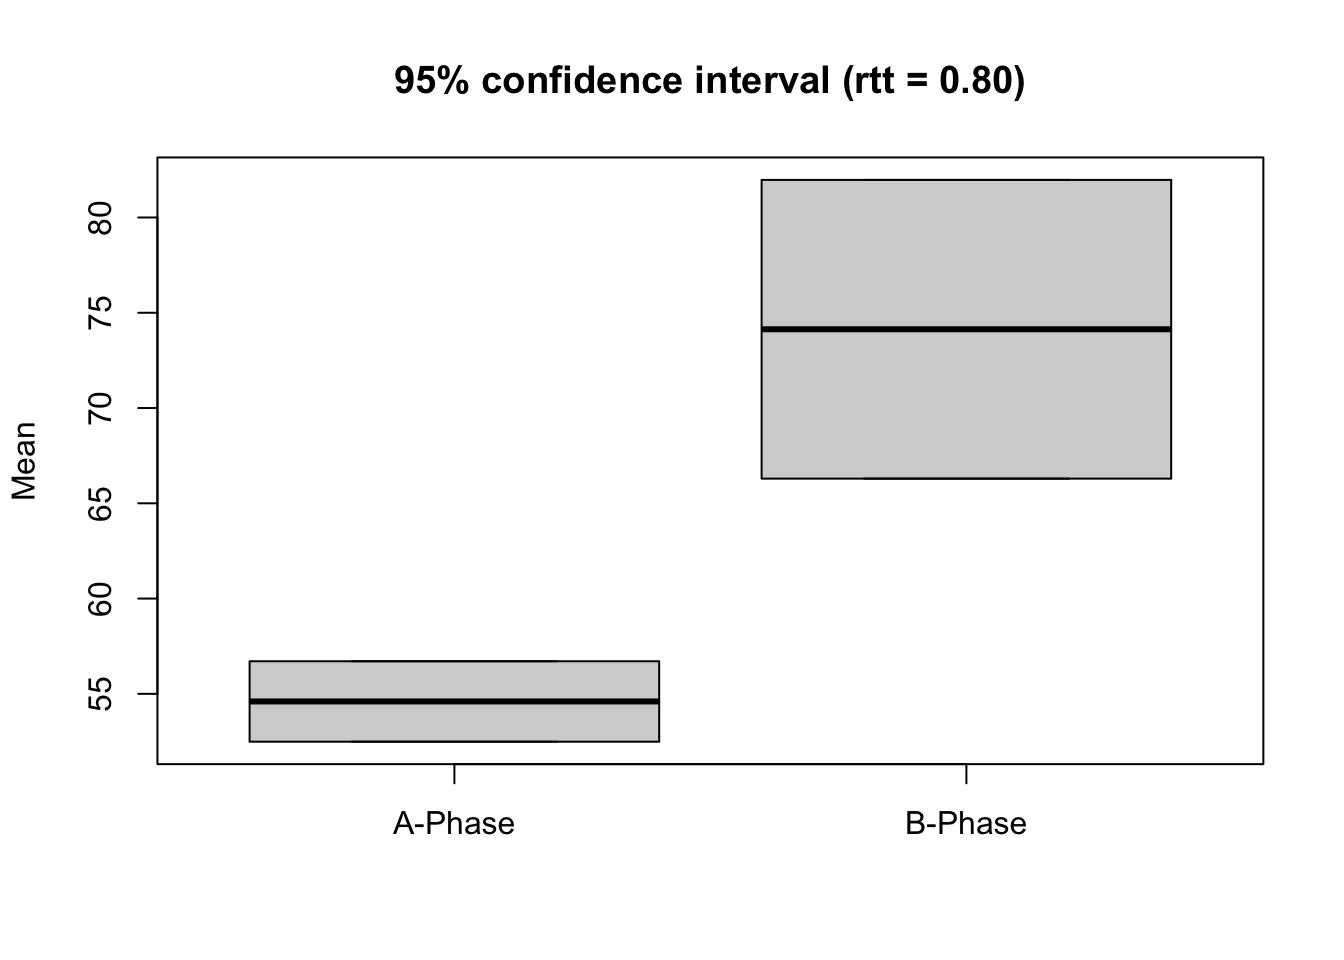
\includegraphics{scan-book_files/figure-latex/unnamed-chunk-39-1.pdf}

\begin{verbatim}
Reliable Change Index

Mean Difference =  19.53333 
Standardized Difference =  1.678301 

Descriptives:
         n     mean       SD       SE
A-Phase  5 54.60000 2.408319 1.077033
B-Phase 15 74.13333 8.943207 3.999524

Reliability =  0.8 

95 % Confidence Intervals:
           Lower    Upper
A-Phase 52.48905 56.71095
B-Phase 66.29441 81.97226

Reliable Change Indices:
                             RCI
Jacobson et al.         18.13624
Christensen and Mendoza 12.82426
Hageman and Arrindell   18.49426
\end{verbatim}

\hypertarget{piecewise-linear-regressions}{%
\chapter{Piecewise linear regressions}\label{piecewise-linear-regressions}}

In a piecewise regression analysis (sometimes called segmented regression) a data-set is split at a specific break point and regression parameters (intercept and slopes) are calculated separately for data before and after the break point. This is done because we assume that at the break point a qualitative change happens affecting intercept and slope. This approach lends itself perfectly to analyze single-case data which are from a statistical point of view time-series data segmented into phases. A general model for single-case data based on the piecewise regression approach has been suggested by Huitema and McKean \protect\hyperlink{ref-huitema_design_2000}{Huitema \& Mckean} (\protect\hyperlink{ref-huitema_design_2000}{2000}). They refer to two-phase single-case designs with a pre-intervention phase containing some measurements before the start of the intervention (A-phase) and an intervention phase containing measurements beginning at the intervention's start and lasting throughout the intervention (B-phase).

In this model, four parameters predict the outcome at a specific measurement point:

\begin{enumerate}
\def\labelenumi{\arabic{enumi}.}
\item
  The performance at the beginning of the study (\textbf{intercept}),
\item
  a developmental effect leading to a continuous increase throughout all measurements (\textbf{trend effect}),
\item
  an intervention effect leading to an immediate and constant increase in performance (l\textbf{evel effect}), and
\item
  a second intervention effect that evolves continuously with the beginning of the intervention (\textbf{slope effect}).
\end{enumerate}

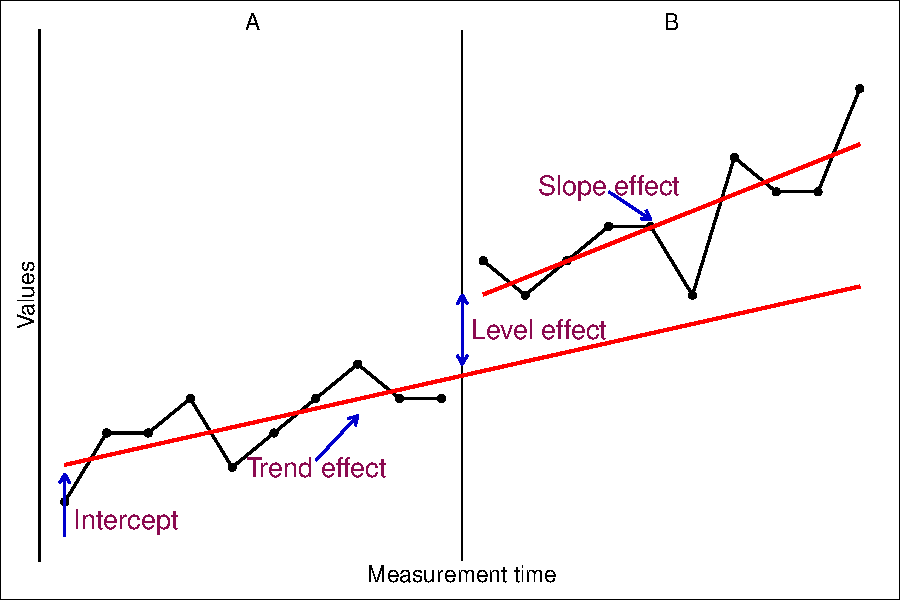
\includegraphics{scan-book_files/figure-latex/figure_plm-1.pdf}

\emph{scan} provides an implementation based on this piecewise regression approach. Though the original model is extended by several factors:

\begin{itemize}
\tightlist
\item
  multiple phase designs
\item
  additional (control) variables
\item
  autoregression modeling
\item
  logistic, binomial, and poisson distributed dependent variables and error terms
\item
  multivariate analyzes for analyzing the effect of an intervention on more than one outcome variable.
\end{itemize}

\hypertarget{the-basic-plm-function}{%
\section{The basic plm function}\label{the-basic-plm-function}}

The basic function for applying a regression analyzes to a single-case dataset is \texttt{plm}. This function analyzes one single-case. In its simplest way, \texttt{plm} takes one argument with an \emph{scdf} object and it returns a full piecewise regression analyzes.

\begin{Shaded}
\begin{Highlighting}[]
\FunctionTok{plm}\NormalTok{(exampleAB}\SpecialCharTok{$}\NormalTok{Johanna)}
\end{Highlighting}
\end{Shaded}

\begin{verbatim}
Piecewise Regression Analysis

Dummy model:  B&L-B 

Fitted a gaussian distribution.
F(3, 16) = 28.69; p = 0.000; R² = 0.843; Adjusted R² = 0.814
\end{verbatim}

\begin{verbatim}
Warning in do.call(data.frame, c(x, alis)): unable to translate '<U+0394>R²' to
native encoding
\end{verbatim}

\begin{verbatim}
                   B   2.5%  97.5%    SE      t     p <U+0394>R²
Intercept     54.300 43.978 64.622 5.267 10.310 0.000           
Trend mt       0.100 -3.012  3.212 1.588  0.063 0.951     0.0000
Level phase B  6.333 -2.979 15.646 4.751  1.333 0.201     0.0174
Slope phase B  1.525 -1.642  4.692 1.616  0.944 0.359     0.0087

Autocorrelations of the residuals
 lag    cr
   1 -0.32
   2 -0.13
   3 -0.01

Formula: values ~ 1 + mt + phaseB + interB
\end{verbatim}

\hypertarget{dummy-model}{%
\subsection{Dummy model}\label{dummy-model}}

The \texttt{model} argument is used to code the \emph{dummy variable}. This \emph{dummy variable} is used to compute the slope and level effects of the \emph{phase} variable.\\
The \emph{phase} variable is categorical, identifying the phase of each measurement. Typically, categorical variables are implemented by means of dummy variables. In a piecewise regression model two phase effects have to be estimated: a level effect and a slope effect. The level effect is implemented quite straight forward: for each phase beginning with the second phase a new dummy variable is created with values of zero for all measurements except the measurements of the phase in focus where values of one are set.

\begin{tabular}{l|r|r}
\hline
phase & values & level\_B\\
\hline
A & 3 & 0\\
\hline
A & 6 & 0\\
\hline
A & 4 & 0\\
\hline
A & 7 & 0\\
\hline
B & 5 & 1\\
\hline
B & 3 & 1\\
\hline
B & 4 & 1\\
\hline
B & 6 & 1\\
\hline
B & 3 & 1\\
\hline
\end{tabular}

For estimating the \emph{slope effect} of each phase, another kind of dummy variables have to be created. Like the dummy variables for level effects the values are set to zero for all measurements except the ones of the phase in focus. Here, values start to increase with every measurement until the end of the phase.\\
Various suggestions have been made regarding the way in which these values increase. The \emph{B\&L-B} model starts with a one at the first measurement of the phase and increases with every measurement while the \emph{H-M} model starts with a zero.

\begin{tabular}{l|r|r|r|r}
\hline
phase & values & level & slope B\&L-M & slope H-M\\
\hline
A & 3 & 0 & 0 & 0\\
\hline
A & 6 & 0 & 0 & 0\\
\hline
A & 4 & 0 & 0 & 0\\
\hline
A & 7 & 0 & 0 & 0\\
\hline
B & 5 & 1 & 1 & 0\\
\hline
B & 3 & 1 & 2 & 1\\
\hline
B & 4 & 1 & 3 & 2\\
\hline
B & 6 & 1 & 4 & 3\\
\hline
B & 3 & 1 & 5 & 4\\
\hline
\end{tabular}

With single-case studies with more than two phases it gets a bit more complicated. Applying the a fore described models to three phases would result in a comparison of each phase to the first phase (usually the A Phase). That is, regression weights and significance tests will depict differences of each phase to the values of phase A. This might be OK depending on what you are interested in. But in a lot of cases we are more interested in analyzing the effects of a phase compared to the previous one.\\
This is achieved applying the \emph{JW} dummy model. In this model, the dummy variable for the level effect is set to zero for all phases preceding the phase in focus and set to one for all remaining measurements. Similar, the dummy variable for the slope effect is set to zero for all phases preceding the one in focus and starts with one for the first measurement of the target phase and increases until the last measurement of the case.

\begin{tabular}{l|r|r|r|r|r}
\hline
phase & values & level\_B & level\_C & slope\_B & slope\_C\\
\hline
A & 3 & 0 & 0 & 0 & 0\\
\hline
A & 6 & 0 & 0 & 0 & 0\\
\hline
A & 4 & 0 & 0 & 0 & 0\\
\hline
A & 7 & 0 & 0 & 0 & 0\\
\hline
B & 5 & 1 & 0 & 1 & 0\\
\hline
B & 3 & 1 & 0 & 2 & 0\\
\hline
B & 4 & 1 & 0 & 3 & 0\\
\hline
B & 6 & 1 & 0 & 4 & 0\\
\hline
B & 3 & 1 & 0 & 5 & 0\\
\hline
C & 7 & 1 & 1 & 6 & 1\\
\hline
C & 5 & 1 & 1 & 7 & 2\\
\hline
C & 6 & 1 & 1 & 8 & 3\\
\hline
C & 4 & 1 & 1 & 9 & 4\\
\hline
C & 8 & 1 & 1 & 10 & 5\\
\hline
\end{tabular}

\hypertarget{adjusting-the-model}{%
\subsection{Adjusting the model}\label{adjusting-the-model}}

\begin{Shaded}
\begin{Highlighting}[]
\NormalTok{example }\OtherTok{\textless{}{-}} \FunctionTok{scdf}\NormalTok{(}
   \AttributeTok{values =} \FunctionTok{c}\NormalTok{(}\DecValTok{55}\NormalTok{, }\DecValTok{58}\NormalTok{, }\DecValTok{53}\NormalTok{, }\DecValTok{50}\NormalTok{, }\DecValTok{52}\NormalTok{, }\DecValTok{55}\NormalTok{, }\DecValTok{68}\NormalTok{, }\DecValTok{68}\NormalTok{, }\DecValTok{81}\NormalTok{, }\DecValTok{67}\NormalTok{, }\DecValTok{78}\NormalTok{, }\DecValTok{73}\NormalTok{, }\DecValTok{72}\NormalTok{, }\DecValTok{78}\NormalTok{, }\DecValTok{81}\NormalTok{, }\DecValTok{78}\NormalTok{, }\DecValTok{71}\NormalTok{, }\DecValTok{85}\NormalTok{, }\DecValTok{80}\NormalTok{, }\DecValTok{76}\NormalTok{),}
   \AttributeTok{phase.design =} \FunctionTok{c}\NormalTok{(}\AttributeTok{A =} \DecValTok{5}\NormalTok{, }\AttributeTok{B =} \DecValTok{15}\NormalTok{)}
\NormalTok{)}

\FunctionTok{plm}\NormalTok{(example)}
\end{Highlighting}
\end{Shaded}

\begin{verbatim}
Piecewise Regression Analysis

Dummy model:  B&L-B 

Fitted a gaussian distribution.
F(3, 16) = 21.36; p = 0.000; R² = 0.800; Adjusted R² = 0.763
\end{verbatim}

\begin{verbatim}
Warning in do.call(data.frame, c(x, alis)): unable to translate '<U+0394>R²' to
native encoding
\end{verbatim}

\begin{verbatim}
                   B   2.5%  97.5%    SE      t     p <U+0394>R²
Intercept     57.800 46.521 69.079 5.755 10.044 0.000           
Trend mt      -1.400 -4.801  2.001 1.735 -0.807 0.432     0.0081
Level phase B 14.467  4.291 24.642 5.192  2.786 0.013     0.0970
Slope phase B  2.500 -0.961  5.961 1.766  1.416 0.176     0.0250

Autocorrelations of the residuals
 lag    cr
   1 -0.28
   2  0.05
   3 -0.11

Formula: values ~ 1 + mt + phaseB + interB
\end{verbatim}

The piecewise regression reveals a significant level effect and two non significant effects for trend and slope. In a further analyses we would like to put the slope effect out of the equation. There are several ways to do this. The easiest way is the to unset the \texttt{slope} argument: \texttt{slope\ =\ FALSE}.

\begin{Shaded}
\begin{Highlighting}[]
\FunctionTok{plm}\NormalTok{(example, }\AttributeTok{slope =} \ConstantTok{FALSE}\NormalTok{)}
\end{Highlighting}
\end{Shaded}

\begin{verbatim}
Piecewise Regression Analysis

Dummy model:  B&L-B 

Fitted a gaussian distribution.
F(2, 17) = 29.30; p = 0.000; R² = 0.775; Adjusted R² = 0.749
\end{verbatim}

\begin{verbatim}
Warning in do.call(data.frame, c(x, alis)): unable to translate '<U+0394>R²' to
native encoding
\end{verbatim}

\begin{verbatim}
                   B   2.5%  97.5%    SE      t     p <U+0394>R²
Intercept     50.559 45.239 55.878 2.714 18.627 0.000           
Trend mt       1.014  0.364  1.664 0.332  3.057 0.007     0.1236
Level phase B 10.329  1.674 18.983 4.416  2.339 0.032     0.0724

Autocorrelations of the residuals
 lag    cr
   1 -0.07
   2  0.06
   3 -0.17

Formula: values ~ 1 + mt + phaseB
\end{verbatim}

In the resulting estimations the trend and level effects are now significant. The model estimated a trend effect of 1.01 points per measurement time and a level effect of 2.46 points. That is, with the beginning of the intervention (the B-phase) the score increases by 15.38 points (5 x 1.01 + 10.33).

\hypertarget{adding-additional-predictors}{%
\subsection{Adding additional predictors}\label{adding-additional-predictors}}

In more complex analyses additional predictors can be included in the piecewise regression model.

To do this, we have to change the regression formula `manually' by applying the \texttt{update} argument. The \texttt{update} argument allows to change the underlying regression formula. To add a new variable named for example \texttt{newVar}, set \texttt{update\ =\ .\textasciitilde{}.\ +\ newVar}. The \texttt{.\textasciitilde{}.} part takes the internally build formula and \texttt{+\ newVar} adds a variable named \texttt{newVar} to the equation.

\begin{Shaded}
\begin{Highlighting}[]
\FunctionTok{plm}\NormalTok{(exampleAB\_add, }\AttributeTok{update =}\NormalTok{ .}\SpecialCharTok{\textasciitilde{}}\NormalTok{. }\SpecialCharTok{+}\NormalTok{ cigarrets)}
\end{Highlighting}
\end{Shaded}

\begin{verbatim}
Piecewise Regression Analysis

Dummy model:  B&L-B 

Fitted a gaussian distribution.
F(4, 35) = 5.87; p = 0.001; R² = 0.402; Adjusted R² = 0.333
\end{verbatim}

\begin{verbatim}
Warning in do.call(data.frame, c(x, alis)): unable to translate '<U+0394>R²' to
native encoding
\end{verbatim}

\begin{verbatim}
                            B   2.5%  97.5%    SE      t     p <U+0394>R²
Intercept              48.579 42.539 54.618 3.081 15.765 0.000           
Trend day               0.392 -0.221  1.005 0.313  1.253 0.218     0.0269
Level phase Medication  3.753 -2.815 10.321 3.351  1.120 0.270     0.0214
Slope phase Medication -0.294 -0.972  0.384 0.346 -0.850 0.401     0.0124
cigarrets              -0.221 -1.197  0.755 0.498 -0.443 0.660     0.0034

Autocorrelations of the residuals
 lag    cr
   1  0.20
   2 -0.19
   3 -0.16

Formula: wellbeing ~ day + phaseMedication + interMedication + cigarrets
\end{verbatim}

The formula has two parts divided by a tilde. Left of the tilde is the variable to be predicted and right of it the predictors. A \texttt{1} indicates the intercept, the variable \texttt{mt} estimates the trend effect, \texttt{phaseB} the level effect of the B-phase and the variable \texttt{interB} the slope effect of the B-phase. If \texttt{formula} is not explicitly defined it is set to \texttt{formula\ =\ values\ \textasciitilde{}\ 1\ +\ mt\ +\ phaseB\ +\ interB} (assuming an AB-design) to estimate the full piecewise regression model.

\hypertarget{to-be-written-modelling-autoregression}{%
\subsection{{[}to be written{]} Modelling autoregression}\label{to-be-written-modelling-autoregression}}

\begin{Shaded}
\begin{Highlighting}[]
\FunctionTok{autocorr}\NormalTok{(Grosche2011)}
\end{Highlighting}
\end{Shaded}

\begin{verbatim}
Autocorrelations

  case phase lag_1 lag_2 lag_3
   Eva     A -0.04 -0.56 -0.01
   Eva     B  0.46  0.10  0.16
   Eva   all  0.48  0.13  0.24
 Georg     A  0.51 -0.01 -0.13
 Georg     B -0.01 -0.02 -0.14
 Georg   all  0.40  0.15 -0.12
  Olaf     A  0.64  0.29 -0.24
  Olaf     B -0.45 -0.20  0.16
  Olaf   all  0.35  0.12 -0.09
\end{verbatim}

\hypertarget{to-be-written-multivariate-piecewise-regression}{%
\section{{[}to be written{]} Multivariate piecewise regression}\label{to-be-written-multivariate-piecewise-regression}}

\begin{Shaded}
\begin{Highlighting}[]
\FunctionTok{mplm}\NormalTok{(exampleAB\_add, }\AttributeTok{dvar =} \FunctionTok{c}\NormalTok{(}\StringTok{"wellbeing"}\NormalTok{, }\StringTok{"depression"}\NormalTok{))}
\end{Highlighting}
\end{Shaded}

\begin{verbatim}
This function is in an experimental state and only implemented for testing und debugging purposes.
\end{verbatim}

\begin{verbatim}
Multivariate piecewise linear model

Dummy model: B&L-B 

Coefficients: 
                        wellbeing depression
(Intercept)            48.0380952  4.0857143
day                     0.3785714  0.1142857
Level Phase Medication  3.8633333 -0.7800000
Slope Phase Medication -0.2754945 -0.1650549

Standardized coefficients: 
                        wellbeing depression
(Intercept)             0.0000000  0.0000000
day                     0.6937874  0.4412216
Level Phase Medication  0.2969359 -0.1262936
Slope Phase Medication -0.3714101 -0.4687655

Formula: y ~ 1 + day + phaseMedication + interMedication

Type III MANOVA Tests: Pillai test statistic
                       Df test stat approx F num Df den Df Pr(>F)    
(Intercept)             1   0.89679  152.053      2     35 <2e-16 ***
day                     1   0.05450    1.009      2     35 0.3750    
Level Phase Medication  1   0.03846    0.700      2     35 0.5034    
Slope Phase Medication  1   0.03911    0.712      2     35 0.4975    
---
Signif. codes:  0 '***' 0.001 '**' 0.01 '*' 0.05 '.' 0.1 ' ' 1
\end{verbatim}

\hypertarget{multilevel-plm-analyses}{%
\section{Multilevel plm analyses}\label{multilevel-plm-analyses}}

Multilevel analyses can take the piecewise-regression approach even further. It allows for

\begin{itemize}
\tightlist
\item
  analyzing the effects between phases for multiple single-cases at once
\item
  describing variability between subjects regarding these effects, and
\item
  introducing variables and factors for explaining the differences.
\end{itemize}

The basic function for applying a multilevel piecewise regression analysis is \texttt{hplm}. The \texttt{hplm} function is similar to the \texttt{plm} function, so I recommend that you get familar with \texttt{plm} before applying an \texttt{hplm}.

Here is a simple example:

\begin{Shaded}
\begin{Highlighting}[]
\FunctionTok{hplm}\NormalTok{(exampleAB\_50)}
\end{Highlighting}
\end{Shaded}

\begin{verbatim}
Hierarchical Piecewise Linear Regression

Estimation method ML 
Slope estimation method: B&L-B 
50 Cases

ICC = 0.195; L = 192.0; p = 0.000

Fixed effects (values ~ 1 + mt + phaseB + interB)

                   B    SE   df      t p
Intercept     51.614 1.282 1281 40.274 0
Trend mt       0.671 0.115 1281  5.844 0
Level phase B 12.938 0.590 1281 21.942 0
Slope phase B  0.859 0.119 1281  7.236 0

Random effects (~1 | case)

          EstimateSD
Intercept      8.179
Residual       5.335
\end{verbatim}

Here is an example inlcuding random slopes:

\begin{Shaded}
\begin{Highlighting}[]
\FunctionTok{hplm}\NormalTok{(exampleAB\_50, }\AttributeTok{random.slopes =} \ConstantTok{TRUE}\NormalTok{)}
\end{Highlighting}
\end{Shaded}

\begin{verbatim}
Hierarchical Piecewise Linear Regression

Estimation method ML 
Slope estimation method: B&L-B 
50 Cases

ICC = 0.195; L = 192.0; p = 0.000

Fixed effects (values ~ 1 + mt + phaseB + interB)

                   B    SE   df      t p
Intercept     51.720 1.348 1281 38.378 0
Trend mt       0.637 0.125 1281  5.080 0
Level phase B 13.090 0.762 1281 17.176 0
Slope phase B  0.887 0.129 1281  6.856 0

Random effects (~1 + mt + phaseB + interB | case)

              EstimateSD
Intercept          8.691
Trend mt           0.343
Level phase B      3.654
Slope phase B      0.358
Residual           4.994
\end{verbatim}

\hypertarget{adding-additional-l2-variables}{%
\subsection{Adding additional L2-variables}\label{adding-additional-l2-variables}}

In some analyses researchers want to investigate whether attributes of the individuals contribute to the effectiveness of an intervention. For example might an intervention on mathematical abilities be less effective for student with a migration background due to too much language related material within the training. Such analyses can also be conducted with \emph{scan}. Therefore, we need to define a new \emph{data frame} including the relevant information of the subjects of the single-case studies we want to analyze. This \emph{data frame} consists of a variable labeled \texttt{case} which has to correspond to the case names of the \emph{scfd} and further variables with attributes of the subjects. To build a \emph{data frame} we can use the R function \texttt{data.frame}.

\begin{Shaded}
\begin{Highlighting}[]
\NormalTok{L2 }\OtherTok{\textless{}{-}} \FunctionTok{data.frame}\NormalTok{(}
  \AttributeTok{case =} \FunctionTok{c}\NormalTok{(}\StringTok{"Antonia"}\NormalTok{,}\StringTok{"Theresa"}\NormalTok{, }\StringTok{"Charlotte"}\NormalTok{, }\StringTok{"Luis"}\NormalTok{, }\StringTok{"Bennett"}\NormalTok{, }\StringTok{"Marie"}\NormalTok{), }
  \AttributeTok{age =} \FunctionTok{c}\NormalTok{(}\DecValTok{16}\NormalTok{, }\DecValTok{13}\NormalTok{, }\DecValTok{13}\NormalTok{, }\DecValTok{10}\NormalTok{, }\DecValTok{5}\NormalTok{, }\DecValTok{14}\NormalTok{), }
  \AttributeTok{sex =} \FunctionTok{c}\NormalTok{(}\StringTok{"f"}\NormalTok{,}\StringTok{"f"}\NormalTok{,}\StringTok{"f"}\NormalTok{,}\StringTok{"m"}\NormalTok{,}\StringTok{"m"}\NormalTok{,}\StringTok{"f"}\NormalTok{)}
\NormalTok{)}
\NormalTok{L2}
\end{Highlighting}
\end{Shaded}

\begin{verbatim}
       case age sex
1   Antonia  16   f
2   Theresa  13   f
3 Charlotte  13   f
4      Luis  10   m
5   Bennett   5   m
6     Marie  14   f
\end{verbatim}

Multilevel analyses require a high number of Level 2 units. The exact number depends on the complexity of the analyses, the size of the effects, the number of level 1 units, and the variability of the residuals. But surely we need at least about 30 level 2 units. In a single-case design that is, we need at least 30 single-cases (subjects) within the study. After setting the level 2 data frame we use the \texttt{data.l2} argument of the \texttt{hplm} function to include it into the analysis. Then we have to specify the regression function using the \texttt{update.fixed} argument. The level 2 variables can be added just like any other additional variable. For example, we have added a level 2 data-set with the two variables \texttt{sex} and \texttt{age}. \texttt{update} could be construed of the level 1 piecewise regression model \texttt{.\textasciitilde{}.} plus the additional level 2 variables of interest \texttt{+\ sex\ +\ age}. The complete argument is \texttt{update.fixed\ =\ .\textasciitilde{}.\ +\ sex\ +\ age}. This analyses will estimate a main effect of sex and age on the overall performance. In case we want to analyze an interaction between the intervention effects and for example the sex of the subject we have to add an additional interaction term (a cross-level interaction). An interaction is defined with a colon. So \texttt{sex:phase} indicates an interaction of sex and the level effect in the single case study. The complete formula now is \texttt{update.fixed\ =\ .\textasciitilde{}.\ +\ sex\ +\ age\ +\ sex:phase}.

\emph{scan} includes an example single-case study with 50 subjects \texttt{example50} and an additional level 2 data-set \texttt{example50.l2}. Here are the first 10 cases of \texttt{example50.l2}.

\begin{tabular}{l|l|r}
\hline
case & sex & age\\
\hline
Jeremiah & m & 10\\
\hline
Leon & m & 12\\
\hline
Pablo & m & 10\\
\hline
Jamal & m & 10\\
\hline
Giovanny & m & 11\\
\hline
Callum & m & 10\\
\hline
Dwayne & m & 11\\
\hline
Neymar & m & 10\\
\hline
Krish & m & 11\\
\hline
Caiden & m & 12\\
\hline
\end{tabular}

Analyzing the data with \texttt{hplm} could look like this:

\begin{Shaded}
\begin{Highlighting}[]
\FunctionTok{hplm}\NormalTok{(exampleAB\_50, }\AttributeTok{data.l2 =}\NormalTok{ exampleAB\_50.l2, }\AttributeTok{update.fixed =}\NormalTok{ .}\SpecialCharTok{\textasciitilde{}}\NormalTok{. }\SpecialCharTok{+}\NormalTok{ sex }\SpecialCharTok{+}\NormalTok{ age)}
\end{Highlighting}
\end{Shaded}

\begin{verbatim}
Hierarchical Piecewise Linear Regression

Estimation method ML 
Slope estimation method: B&L-B 
50 Cases

ICC = 0.195; L = 192.0; p = 0.000

Fixed effects (values ~ mt + phaseB + interB + sex + age)

                   B     SE   df      t     p
Intercept     71.464 13.076 1281  5.465 0.000
Trend mt       0.667  0.115 1281  5.808 0.000
Level phase B 12.951  0.590 1281 21.951 0.000
Slope phase B  0.863  0.119 1281  7.264 0.000
sexm          -2.130  2.336   47 -0.912 0.367
age           -1.710  1.157   47 -1.478 0.146

Random effects (~1 | case)

          EstimateSD
Intercept      7.975
Residual       5.335
\end{verbatim}

\texttt{sex} is a factor with the levels \texttt{f} and \texttt{m}. So \texttt{sexm} is the effect of being male on the overall performance. \texttt{age} does not seem to have any effect. So we drop \texttt{age} out of the equation and add an interaction of sex and phase to see whether the \texttt{sex} effect is due to a weaker impact of the intervention on males.

\begin{Shaded}
\begin{Highlighting}[]
\FunctionTok{hplm}\NormalTok{(exampleAB\_50, }\AttributeTok{data.l2 =}\NormalTok{ exampleAB\_50.l2, }\AttributeTok{update.fixed =}\NormalTok{ .}\SpecialCharTok{\textasciitilde{}}\NormalTok{. }\SpecialCharTok{+}\NormalTok{ sex }\SpecialCharTok{+}\NormalTok{ sex}\SpecialCharTok{:}\NormalTok{phaseB)}
\end{Highlighting}
\end{Shaded}

\begin{verbatim}
Hierarchical Piecewise Linear Regression

Estimation method ML 
Slope estimation method: B&L-B 
50 Cases

ICC = 0.195; L = 192.0; p = 0.000

Fixed effects (values ~ mt + phaseB + interB + sex + phaseB:sex)

                        B    SE   df       t     p
Intercept          49.801 1.735 1280  28.711 0.000
Trend mt            0.638 0.109 1280   5.847 0.000
Level phase B      16.762 0.644 1280  26.034 0.000
Slope phase B       0.889 0.113 1280   7.884 0.000
sexm                3.983 2.368   48   1.682 0.099
Level phase B:sexm -7.463 0.622 1280 -11.994 0.000

Random effects (~1 | case)

          EstimateSD
Intercept      8.144
Residual       5.059
\end{verbatim}

Now the interaction \texttt{phase:sexm} is significant and the main effect is no longer relevant. It looks like the intervention effect is 7.5 points lower for male subjects. While the level-effect is 16.8 points for female subjects it is 16.8 - 7.5 = 9.3 for males.

\hypertarget{randomization-tests}{%
\chapter{Randomization tests}\label{randomization-tests}}

The \texttt{rand\_test} function computes a randomization test for single or multiple baseline single-case data. The function is based on an algorithm from the SCRT package (Bulte \& Onghena, 2009, 2012), but rewritten and extended for the use in AB designs.

The \texttt{statsitics} argument defines the statistic on which the comparison of the phases is based on. The following comparisons are possible:

\begin{itemize}
\tightlist
\item
  ``Mean A-B'': Uses the difference between the mean of phase A and the mean of phase B. * This is appropriate if a decrease of scores is expected for phase B.
\item
  ``Mean B-A'': Uses the difference between the mean of phase B and the mean of phase A. This is appropriate if an increase of scores is expected for phase B.
\item
  ``Mean \textbar A-B\textbar{}'': Uses the absolute value of the difference between the means of phases A and B.
\item
  ``Median A-B'': The same as ``Mean A-B,'' but based on the median.
\item
  ``Median B-A'': The same as ``Mean B-A,'' but based on the median.
\end{itemize}

\emph{number}\\
Sample size of the randomization distribution. The exactness of the p-value can not exceed 1/number (i.e., number = 100 results in p-values with an exactness of one percent). Default is number = 500. For faster processing use number = 100. For more precise p-values set number = 1000.

\emph{complete}\\
If TRUE, the distribution is based on a complete permutation of all possible starting combinations. This setting overwrites the number Argument. The default setting is FALSE.

\emph{limit}\\
Minimal number of data points per phase in the sample. The first number refers to the A-phase and the second to the B-phase (e.g., limit = c(5, 3)). If only one number is given, this number is applied to both phases. Default is limit = 5.

\emph{startpoints}\\
Alternative to the limit-parameter, startpoints exactly defines the possible start points of phase B (e.g., startpoints = 4:9 restricts the phase B start points to measurements 4 to 9. startpoints overwrite the limit-parameter.

\emph{exclude.equal}\\
If set to FALSE, which is the default, random distribution values equal to the observed distribution are counted as null-hypothesis conform. That is, they decrease the probability of rejecting the null-hypothesis (increase the p-value). exclude.equal should be set to TRUE if you analyse one single-case design (not a multiple baseline data set) to reach a sufficient power. But be aware, that it increases the chance of an alpha-error.

\emph{graph}\\
If set TRUE, a histogram of the resulting distribution is plotted.

\emph{phases}\\
A vector of two characters or numbers indicating the two phases that should be compared. E.g., phases = c(``A,''``C'') or phases = c(2,4) for comparing the second and the fourth phase. Phases could be combined by providing a list with two elements. E.g., phases = list(A = c(1,3), B = c(2,4)) will compare phases 1 and 3 (as A) against 2 and 4 (as B). Default is phases = c(``A,''``B'').

\begin{Shaded}
\begin{Highlighting}[]
\FunctionTok{rand\_test}\NormalTok{(exampleAB, }\AttributeTok{graph =} \ConstantTok{TRUE}\NormalTok{)}
\end{Highlighting}
\end{Shaded}

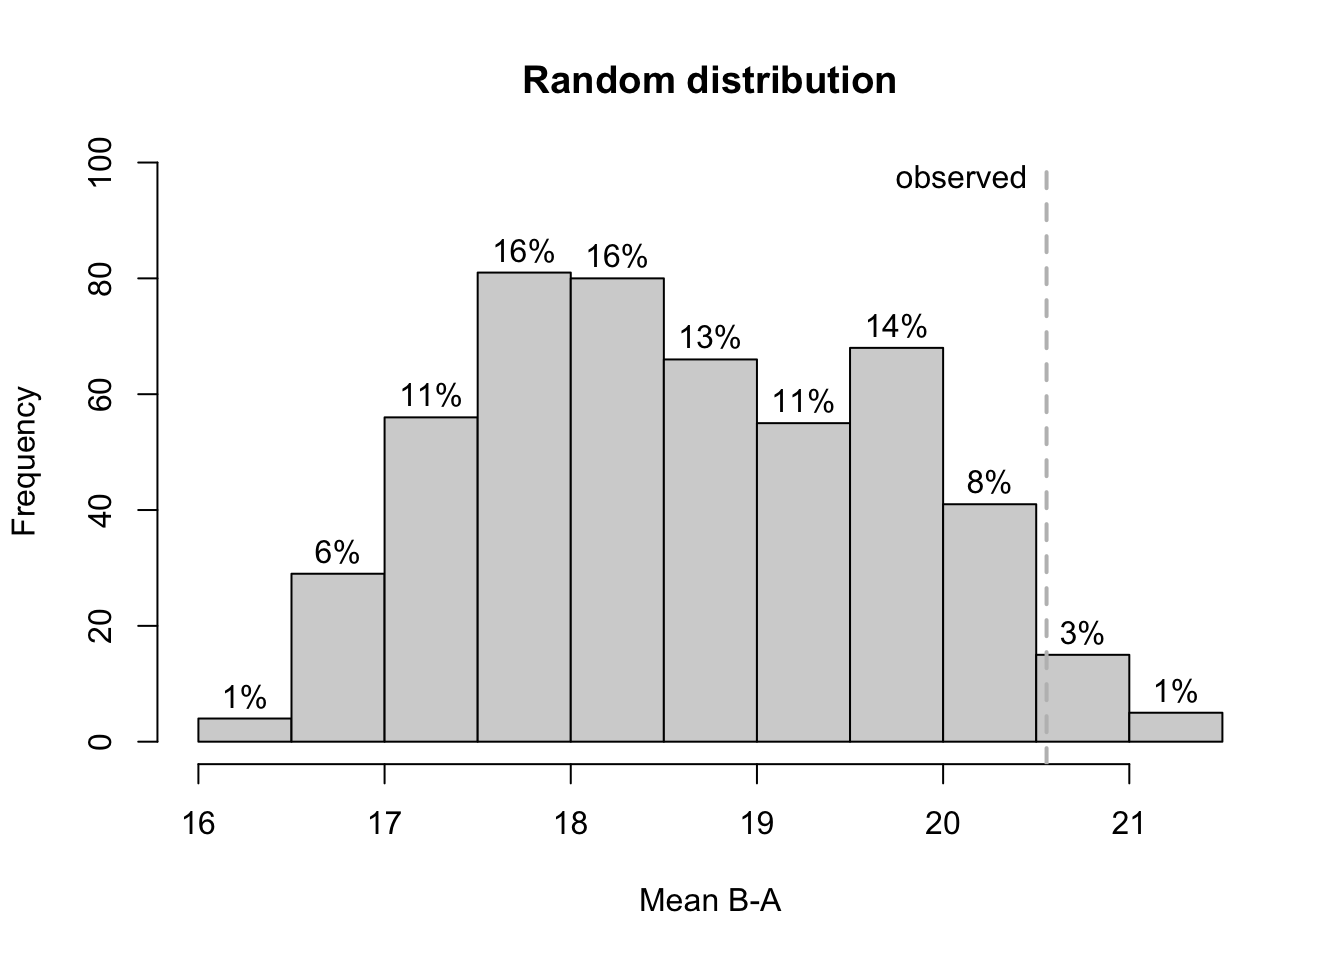
\includegraphics{scan-book_files/figure-latex/rand-1.pdf}

\begin{verbatim}
Randomization Test

Test for 3 cases.

Comparing phase 1 against phase 2 
Statistic:  Mean B-A 

Minimal length of each phase:  5 5 
Observed statistic =  20.55556 


Distribution based on a random sample of all 1331 possible combinations.
n   =  500 
M   =  18.59305 
SD  =  1.114388 
Min =  16.05185 
Max =  21.34493 

p   =  0.036 

Shapiro-Wilk Normality Test: W = 0.979; p = 0.000  (Hypothesis of Normality rejected)
z = 1.7611, p = 0.0391 (single sided)
\end{verbatim}

\hypertarget{default-settings}{%
\chapter{Default settings}\label{default-settings}}

Some of the default settings of scan can be changed with the \texttt{options()} argument. Table \ref{tab:table-options} shows a complete list of options and their default values.

\begin{Shaded}
\begin{Highlighting}[]
\CommentTok{\# get the current value of an option}
\FunctionTok{getOption}\NormalTok{(}\StringTok{"scan.print.rows"}\NormalTok{)}
\end{Highlighting}
\end{Shaded}

\begin{verbatim}
[1] 15
\end{verbatim}

\begin{Shaded}
\begin{Highlighting}[]
\CommentTok{\# set option to a different value}
\FunctionTok{options}\NormalTok{(}\AttributeTok{scan.print.rows =} \DecValTok{5}\NormalTok{, }\AttributeTok{scan.print.scdf.name =} \ConstantTok{FALSE}\NormalTok{)}
\FunctionTok{print}\NormalTok{(exampleAB)}
\end{Highlighting}
\end{Shaded}

\begin{verbatim}
#A single-case data frame with 3 cases

 phase values mt | phase values mt | phase values mt |
     A     54  1 |     A     41  1 |     A     55  1 |
     A     53  2 |     A     59  2 |     A     58  2 |
     A     56  3 |     A     56  3 |     A     53  3 |
     A     58  4 |     A     51  4 |     A     50  4 |
     A     52  5 |     A     52  5 |     A     52  5 |
# ... up to 15 more rows
\end{verbatim}

\begin{Shaded}
\begin{Highlighting}[]
\FunctionTok{options}\NormalTok{(}\AttributeTok{scan.print.rows =} \DecValTok{15}\NormalTok{, }\AttributeTok{scan.print.scdf.name =} \ConstantTok{TRUE}\NormalTok{)}
\FunctionTok{print}\NormalTok{(exampleAB)}
\end{Highlighting}
\end{Shaded}

\begin{verbatim}
#A single-case data frame with 3 cases

 Johanna: phase values mt | Karolina: phase values mt | Anja: phase values mt |
              A     54  1 |               A     41  1 |           A     55  1 |
              A     53  2 |               A     59  2 |           A     58  2 |
              A     56  3 |               A     56  3 |           A     53  3 |
              A     58  4 |               A     51  4 |           A     50  4 |
              A     52  5 |               A     52  5 |           A     52  5 |
              B     61  6 |               B     57  6 |           B     55  6 |
              B     62  7 |               B     56  7 |           B     68  7 |
              B     71  8 |               B     67  8 |           B     68  8 |
              B     66  9 |               B     75  9 |           B     81  9 |
              B     64 10 |               B     66 10 |           B     67 10 |
              B     78 11 |               B     69 11 |           B     78 11 |
              B     70 12 |               B     68 12 |           B     73 12 |
              B     74 13 |               B     73 13 |           B     72 13 |
              B     82 14 |               B     77 14 |           B     78 14 |
              B     77 15 |               B     79 15 |           B     81 15 |
# ... up to 5 more rows
\end{verbatim}

\begin{table}

\caption{\label{tab:table-options}Scan Options}
\centering
\begin{tabular}[t]{>{\raggedright\arraybackslash}p{15em}>{\raggedright\arraybackslash}p{15em}l}
\toprule
Option & Default & What it does ...\\
\midrule
\textbf{scan.print.cases} & "fit" & Max number of cases printed for scdf objects\\
\textbf{scan.print.rows} & 15 & Max number of rows printed for scdf objects\\
\textbf{scan.print.cols} & "all" & Max number of columns printed for scdf objects\\
\textbf{scan.print.digits} & 1 & Max number of digits printed for scdf objects\\
\textbf{scan.print.long} & FALSE & If TRUE, prints scdf objects in long format\\
\addlinespace
\textbf{scan.print.scdf.name} & TRUE & If TRUE, prints case names of scdf\\
\textbf{scan.deprecated.warning} & FALSE & When TRUE returns information on deprecated functions\\
\textbf{scan.export.kable} & list(digits = 2, booktab = TRUE) & List with default arguments for the kable argument of the export function\\
\textbf{scan.export.kable\_styling} & list(bootstrap\_options = c("bordered", "condensed"), full\_width = FALSE, position = "center") & List with default arguments for the kable\_styling argument of the export function\\
\textbf{scan.plot.style} & "grid" & NA\\
\bottomrule
\end{tabular}
\end{table}

\hypertarget{exporting-scan-results}{%
\chapter{\texorpdfstring{Exporting \emph{scan} results}{Exporting scan results}}\label{exporting-scan-results}}

The \texttt{export} function will make it easier to convert the results of your \texttt{scan} analyses into tables and descriptions you can add to your documents and presentations. Basically, \texttt{export} takes a \texttt{scan} object and converts it to an html-table or latex output.

\begin{rmdnote}
\texttt{export} it build on top of the \texttt{knitr} and
\texttt{kableextra} packages. The list provided in the
\texttt{kable\_options} argument is implemented in the \texttt{kable}
function of \texttt{knitr} and the list provided to the
\texttt{kable\_styling\_options} is implemented in the
\texttt{kable\_styling} command of the \texttt{kableExtra} package.
\texttt{export} sets some defaults for these functions but you can play
around and overwrite them.
\end{rmdnote}

\texttt{export} works best when used within an rmarkdown file and/or within \texttt{RStudio}.\\
In \texttt{RStudio}

{[}xxx to be continued!{]}

\hypertarget{single-case-data-files}{%
\section{Single case data files}\label{single-case-data-files}}

\begin{Shaded}
\begin{Highlighting}[]
\FunctionTok{export}\NormalTok{(exampleA1B1A2B2\_zvt)}
\end{Highlighting}
\end{Shaded}

\begin{table}
\centering
\begin{tabular}{cccccccccccc}
\toprule
\multicolumn{4}{c}{Tick} & \multicolumn{4}{c}{Trick} & \multicolumn{4}{c}{Track} \\
\cmidrule(l{3pt}r{3pt}){1-4} \cmidrule(l{3pt}r{3pt}){5-8} \cmidrule(l{3pt}r{3pt}){9-12}
zvt & d2 & day & part & zvt & d2 & day & part & zvt & d2 & day & part\\
\midrule
47 & 131 & 1 & A1 & 51 & 100 & 1 & A1 & 54 & 89 & 1 & A1\\
58 & 134 & 2 & A1 & 58 & 126 & 2 & A1 & 57 & 116 & 2 & A1\\
76 & 141 & 3 & A1 & 70 & 130 & 3 & A1 & 51 & 114 & 3 & A1\\
63 & 141 & 4 & B1 & 65 & 130 & 4 & B1 & 61 & 131 & 4 & B1\\
71 & 140 & 5 & B1 & 67 & 137 & 5 & B1 & 57 & 132 & 5 & B1\\
\addlinespace
59 & 140 & 6 & B1 & 63 & 133 & 6 & B1 & 53 & 130 & 6 & B1\\
64 & 138 & 7 & A2 & 64 & 136 & 7 & A2 & 58 & 128 & 7 & A2\\
69 & 140 & 8 & A2 & 70 & 137 & 8 & A2 & 57 & 131 & 8 & A2\\
72 & 141 & 9 & A2 & 70 & 135 & 9 & A2 & 60 & 130 & 9 & A2\\
77 & 140 & 10 & B2 & 68 & 128 & 10 & B2 & 55 & 129 & 10 & B2\\
\addlinespace
76 & 138 & 11 & B2 & 69 & 137 & 11 & B2 & 58 & 118 & 11 & B2\\
73 & 140 & 12 & B2 & 70 & 138 & 12 & B2 & 58 & 131 & 12 & B2\\
\bottomrule
\end{tabular}
\end{table}

\hypertarget{descriptive-stats}{%
\section{Descriptive stats}\label{descriptive-stats}}

\begin{Shaded}
\begin{Highlighting}[]
\NormalTok{res }\OtherTok{\textless{}{-}} \FunctionTok{describeSC}\NormalTok{(GruenkeWilbert2014)}
\FunctionTok{export}\NormalTok{(res)}
\end{Highlighting}
\end{Shaded}

Descriptive statistics.

\begin{table}
\centering
\begin{tabular}{lcccccccccccccccccc}
\toprule
\multicolumn{1}{c}{ } & \multicolumn{2}{c}{n} & \multicolumn{2}{c}{Missing} & \multicolumn{2}{c}{M} & \multicolumn{2}{c}{Median} & \multicolumn{2}{c}{SD} & \multicolumn{2}{c}{MAD} & \multicolumn{2}{c}{Min} & \multicolumn{2}{c}{Max} & \multicolumn{2}{c}{Trend} \\
\cmidrule(l{3pt}r{3pt}){2-3} \cmidrule(l{3pt}r{3pt}){4-5} \cmidrule(l{3pt}r{3pt}){6-7} \cmidrule(l{3pt}r{3pt}){8-9} \cmidrule(l{3pt}r{3pt}){10-11} \cmidrule(l{3pt}r{3pt}){12-13} \cmidrule(l{3pt}r{3pt}){14-15} \cmidrule(l{3pt}r{3pt}){16-17} \cmidrule(l{3pt}r{3pt}){18-19}
  & A & B & A & B & A & B & A & B & A & B & A & B & A & B & A & B & A & B\\
\midrule
Anton & 4 & 14 & 0 & 0 & 5.00 & 9.14 & 5 & 9 & 0.82 & 0.77 & 0.74 & 1.48 & 4 & 8 & 6 & 10 & -0.40 & 0.03\\
Bob & 7 & 11 & 0 & 0 & 3.00 & 8.82 & 3 & 9 & 0.82 & 0.87 & 1.48 & 0.00 & 2 & 7 & 4 & 10 & 0.04 & 0.04\\
Paul & 6 & 12 & 0 & 0 & 3.83 & 8.83 & 4 & 9 & 0.75 & 0.72 & 0.74 & 0.74 & 3 & 8 & 5 & 10 & -0.26 & 0.02\\
Robert & 8 & 10 & 0 & 0 & 4.12 & 8.90 & 4 & 9 & 0.83 & 0.99 & 1.48 & 1.48 & 3 & 7 & 5 & 10 & -0.06 & -0.14\\
Sam & 5 & 13 & 0 & 0 & 4.60 & 9.08 & 5 & 9 & 0.55 & 0.86 & 0.00 & 1.48 & 4 & 8 & 5 & 10 & 0.10 & 0.03\\
\addlinespace
Tim & 4 & 14 & 0 & 0 & 3.00 & 9.00 & 3 & 9 & 0.82 & 0.96 & 0.74 & 1.48 & 2 & 7 & 4 & 10 & -0.60 & 0.00\\
\bottomrule
\end{tabular}
\end{table}

n = Number of measurements; Missing = Number of missing values; M = Mean; Median = Median; SD = Standard deviation; MAD = Median average deviation; Min = Minimum; Max = Maximum; Trend = Slope of dependent variable regressed on measurement-time.

\hypertarget{overlap-indices}{%
\section{Overlap indices}\label{overlap-indices}}

\begin{Shaded}
\begin{Highlighting}[]
\NormalTok{res }\OtherTok{\textless{}{-}} \FunctionTok{overlap}\NormalTok{(exampleA1B1A2B2\_zvt, }\AttributeTok{phases =} \FunctionTok{list}\NormalTok{(}\FunctionTok{c}\NormalTok{(}\DecValTok{1}\NormalTok{,}\DecValTok{3}\NormalTok{),}\FunctionTok{c}\NormalTok{(}\DecValTok{2}\NormalTok{,}\DecValTok{4}\NormalTok{)))}
\FunctionTok{export}\NormalTok{(res, }\AttributeTok{flip =} \ConstantTok{TRUE}\NormalTok{)}
\end{Highlighting}
\end{Shaded}

Overlap indices.Comparing phases A1 + A2 against phases B1 + B2.

\begin{table}
\centering
\begin{tabular}{lrrr}
\toprule
  & Tick & Trick & Track\\
\midrule
PND & 16.67 & 0.00 & 16.67\\
PEM & 66.67 & 50.00 & 50.00\\
PET & 66.67 & 33.33 & 33.33\\
NAP & 68.06 & 51.39 & 58.33\\
NAP-R & 36.11 & 2.78 & 16.67\\
\addlinespace
PAND & 66.67 & 50.00 & 54.17\\
Tau-U & 0.14 & 0.03 & -0.03\\
Base\_Tau & 0.27 & 0.02 & 0.13\\
Delta M & 5.50 & 3.17 & 0.83\\
Delta Trend & -0.31 & -1.10 & -0.74\\
\addlinespace
SMD & 0.52 & 0.40 & 0.26\\
\bottomrule
\end{tabular}
\end{table}

PND = Percentage Non-Overlapping Data; PEM = Percentage Exceeding the Median; PET = Percentage Exceeding the Trend; NAP = Nonoverlap of all pairs; NAP-R = NAP rescaled;
PAND = Percentage all nonoverlapping data;Tau U = Parker's Tau-U; Base Tau = Baseline corrected Tau; Delta M = Mean difference between phases; Delta Trend = Trend difference between phases; SMD = Standardized Mean Difference.

\hypertarget{piecewise-linear-models}{%
\section{Piecewise linear models}\label{piecewise-linear-models}}

\begin{Shaded}
\begin{Highlighting}[]
\NormalTok{res }\OtherTok{\textless{}{-}} \FunctionTok{plm}\NormalTok{(exampleA1B1A2B2}\SpecialCharTok{$}\NormalTok{Pawel)}
\FunctionTok{export}\NormalTok{(res)}
\end{Highlighting}
\end{Shaded}

Piecewise-regression model for variable `values.'

\begin{table}
\centering
\begin{tabular}{lrrrrrrr}
\toprule
\multicolumn{2}{c}{ } & \multicolumn{2}{c}{CI(95\%)} & \multicolumn{4}{c}{ } \\
\cmidrule(l{3pt}r{3pt}){3-4}
Parameter & B & 2.5\% & 97.5\% & SE & t & p & Delta R²\\
\midrule
Intercept & 12.47 & 4.90 & 20.03 & 3.86 & 3.23 & <.01 & \\
Trend mt & 0.22 & -0.99 & 1.44 & 0.62 & 0.36 & .72 & .00\\
Level phase B1 & 17.69 & 7.71 & 27.67 & 5.09 & 3.48 & <.01 & .14\\
Level phase A2 & 2.58 & -16.96 & 22.12 & 9.97 & 0.26 & .79 & .00\\
Level phase B2 & 12.54 & -18.46 & 43.54 & 15.82 & 0.79 & .43 & .01\\
\addlinespace
Slope phase B1 & -1.41 & -3.13 & 0.32 & 0.88 & -1.60 & .11 & .03\\
Slope phase A2 & -1.10 & -2.83 & 0.62 & 0.88 & -1.25 & .21 & .02\\
Slope phase B2 & -1.08 & -2.81 & 0.64 & 0.88 & -1.23 & .22 & .02\\
\bottomrule
\multicolumn{8}{l}{\rule{0pt}{1em}\textit{Note: }}\\
\multicolumn{8}{l}{\rule{0pt}{1em}F(7, 32) = 7.86; p <.001; R² = 0.632; Adjusted R² = 0.552}\\
\end{tabular}
\end{table}

\hypertarget{hierarchical-piecewise-regressions}{%
\section{Hierarchical piecewise regressions}\label{hierarchical-piecewise-regressions}}

\begin{Shaded}
\begin{Highlighting}[]
\NormalTok{res }\OtherTok{\textless{}{-}} \FunctionTok{hplm}\NormalTok{(exampleAB\_50, }\AttributeTok{data.l2 =}\NormalTok{ exampleAB\_50.l2, }\AttributeTok{lr.test =} \ConstantTok{TRUE}\NormalTok{, }\AttributeTok{random.slopes =} \ConstantTok{TRUE}\NormalTok{)}
\FunctionTok{export}\NormalTok{(res)}
\end{Highlighting}
\end{Shaded}

Hierarchical Piecewise Linear Regression for variable `values.'

\begin{table}
\centering
\begin{tabular}{lrrrrr}
\toprule
Parameter & B & SE & df & t & p\\
\midrule
Intercept & 51.72 & 1.35 & 1281 & 38.38 & <.001\\
Trend mt & 0.64 & 0.13 & 1281 & 5.08 & <.001\\
Level phase B & 13.09 & 0.76 & 1281 & 17.18 & <.001\\
Slope phase B & 0.89 & 0.13 & 1281 & 6.86 & <.001\\
\midrule
\addlinespace[0.3em]
\multicolumn{6}{l}{\textbf{Random effects}}\\
\textcolor{black}{\textbf{\hspace{1em}}} & \textcolor{black}{\textbf{SD}} & \textcolor{black}{\textbf{L}} & \textcolor{black}{\textbf{df}} & \textcolor{black}{\textbf{p}} & \textcolor{black}{\textbf{}}\\
\hspace{1em}Intercept & 8.69 & 194.8 & 4 & <.001 & \\
\hspace{1em}Trend mt & 0.34 & 4.8 & 4 & .30 & \\
\hspace{1em}Level phase B & 3.65 & 28.25 & 4 & <.001 & \\
\hspace{1em}Slope phase B & 0.36 & 4.81 & 4 & .30 & \\
\hspace{1em}Residual & 4.99 & NA & NA & NA & \\
\midrule
AIC & 8403.5 &  &  &  & \\
BIC & 8481.5 &  &  &  & \\
ICC & 0.2 & L = 192 & p <.001 &  & \\
\bottomrule
\multicolumn{6}{l}{\rule{0pt}{1em}\textit{Note: }}\\
\multicolumn{6}{l}{\rule{0pt}{1em}Estimation method ML; Slope estimation method: B\&L-B; 50 cases}\\
\end{tabular}
\end{table}

\hypertarget{about-the-author}{%
\chapter*{About the author}\label{about-the-author}}
\addcontentsline{toc}{chapter}{About the author}

Currently, I am a professor for research methods and diagnostics at the department of inclusive education at the University of Potsdam in Germany. I studied education sciences at the University of Cologne where I also did my PhD in psychology. Thereafter, I got a tenured position as a senior researcher at the department of special education (also University of Cologne). Later I did my habilitation on ``Pedagogic and psychology in learning disabilities'' at the \emph{Carl von Ossietzky University} Oldenburg.

My current work focuses on:

\begin{itemize}
\tightlist
\item
  Single-case research designs, analyzing single case data, and reporting single-case based results.
\item
  Social inclusion and social participation in classrooms.
\item
  Implementation of Open Science and Data Science concepts into special education research.
\end{itemize}

My work can be found at:

\begin{itemize}
\tightlist
\item
  University of Potsdam: \url{https://www.uni-potsdam.de/en/inklusion/researchmethodsanddiagnostics/wilbert.html}
\item
  Researchgate: \url{https://www.researchgate.net/profile/Juergen_Wilbert2}
\item
  github: \url{https://github.com/jazznbass}
\item
  orcid: \url{https://orcid.org/0000-0002-8392-2873}
\item
  Googel scholar: \url{https://scholar.google.de/citations?user=RF7Siq4AAAAJ\&hl=en}
\item
  Empirische Sonderpädagogik: \url{http://www.psychologie-aktuell.com/index.php?id=255}
\item
  OSF (Open science framework): \url{https://osf.io/q7gme/}
\end{itemize}

\hypertarget{references}{%
\chapter*{References}\label{references}}
\addcontentsline{toc}{chapter}{References}

\hypertarget{refs}{}
\begin{CSLReferences}{1}{0}
\leavevmode\hypertarget{ref-R-rmarkdown}{}%
Allaire, J., Xie, Y., McPherson, J., Luraschi, J., Ushey, K., Atkins, A., \ldots{} Iannone, R. (2021). \emph{Rmarkdown: Dynamic documents for r}. Retrieved from \url{https://CRAN.R-project.org/package=rmarkdown}

\leavevmode\hypertarget{ref-huitema_design_2000}{}%
Huitema, B. E., \& Mckean, J. W. (2000). Design specification issues in time-series intervention models. \emph{Educational and Psychological Measurement}, \emph{60}(1), 38--58. Retrieved from \url{http://epm.sagepub.com/content/60/1/38.short}

\leavevmode\hypertarget{ref-iglewicz_how_1993}{}%
Iglewicz, B., \& Hoaglin, D. C. (1993). \emph{How to detect and handle outliers}. Milwaukee, Wis. : ASQC Quality Press.

\leavevmode\hypertarget{ref-parker_percentage_2007}{}%
Parker, Richard I., Hagan-Burke, S., \& Vannest, K. (2007). Percentage of {All} {Non}-{Overlapping} {Data} ({PAND}) {An} {Alternative} to {PND}. \emph{The Journal of Special Education}, \emph{40}(4), 194--204. Retrieved from \url{http://sed.sagepub.com/content/40/4/194.short}

\leavevmode\hypertarget{ref-parker_improved_2009}{}%
Parker, Richard I., \& Vannest, K. (2009). An improved effect size for single-case research: {Nonoverlap} of all pairs. \emph{Behavior Therapy}, \emph{40}(4), 357--367. Retrieved from \url{http://www.sciencedirect.com/science/article/pii/S0005789408000816}

\leavevmode\hypertarget{ref-parker_effect_2011}{}%
Parker, Richard I., Vannest, K. J., \& Davis, J. L. (2011). Effect {Size} in {Single}-{Case} {Research}: {A} {Review} of {Nine} {Nonoverlap} {Techniques}. \emph{Behavior Modification}, \emph{35}(4), 303--322. \url{https://doi.org/10.1177/0145445511399147}

\leavevmode\hypertarget{ref-parker_combining_2011}{}%
Parker, Richard I., Vannest, K. J., Davis, J. L., \& Sauber, S. B. (2011). Combining {Nonoverlap} and {Trend} for {Single}-{Case} {Research}: {Tau}-{U}. \emph{Behavior Therapy}, \emph{42}(2), 284--299. \url{https://doi.org/10.1016/j.beth.2010.08.006}

\leavevmode\hypertarget{ref-R-base}{}%
R Core Team. (2021). \emph{R: A language and environment for statistical computing}. Retrieved from \url{https://www.R-project.org/}

\leavevmode\hypertarget{ref-RStudio}{}%
RStudio Team. (2018). \emph{RStudio: Integrated development environment for r}. Retrieved from \url{http://www.rstudio.com/}

\leavevmode\hypertarget{ref-scruggs_quantitative_1987}{}%
Scruggs, T. E., Mastropieri, M. A., \& Casto, G. (1987). The {Quantitative} {Synthesis} of {Single}-{Subject} {Research} {Methodology} and {Validation}. \emph{Remedial and Special Education}, \emph{8}(2), 24--33. \url{https://doi.org/10.1177/074193258700800206}

\leavevmode\hypertarget{ref-R-scan}{}%
Wilbert, J., \& Lueke, T. (2021). \emph{Scan: Single-case data analyses for single and multiple baseline designs}.

\leavevmode\hypertarget{ref-wise_methods_2004}{}%
Wise, E. A. (2004). Methods for analyzing psychotherapy outcomes: {A} review of clinical significance, reliable change, and recommendations for future directions. \emph{Journal of Personality Assessment}, \emph{82}(1), 50--59. Retrieved from \url{http://www.tandfonline.com/doi/abs/10.1207/s15327752jpa8201_10}

\leavevmode\hypertarget{ref-R-bookdown}{}%
Xie, Y. (2020). \emph{Bookdown: Authoring books and technical documents with r markdown}. Retrieved from \url{https://github.com/rstudio/bookdown}

\end{CSLReferences}

\end{document}
